\subsubsection{Bucket}

  \begin{enumerate}
    \item The main requirements for the module were:
  	  \begin{itemize}
        \item Maximum capacity: five cubes and three spheres
        \item A mechanical limiter on the amount of debris in the bucket 
        \item A closing mechanism for the bucket
        \item Delivery mechanism for putting the debris into the goals should work in both directions.  
  	  \end{itemize}  
    \item The first stage of development was creating the general concept of the module, its structure and method of operation. In result, was decided on the following mechanism: 
    The bucket is shifted outside of the robot and turned 90 degrees around an axis parallel to the axis of shift;
    both movements are done by one servo.
    This allows to place the bucket opening to be parallel to the ground and increase the accuracy of debris delivery. Movement in two planes at once is accomplished through sloped guide rails, which turn the beams with the bucket during their sideways movement. To prevent premature release of debris from the bucket, the bucket opening will be closed. 
    
  \item The next step was developing the closing mechanism. To minimize the load on the servo completing the turning movement, the center of mass of the module has to be situated as close as possible to the mounting point on the lifting mechanism. Thus, the following system was developed:
    \begin{itemize}
      \item On the beam which is mounted to the lifting mechanism, is installed a reel with twine.
      \item The twine is fixed in such a way that when the reel turns in one direction, one of the ends is pulled taut while the other  slacks, and vice versa.
      \item The twine wraps around several fixed blocks along all the beams which support the bucket.
      \item Above the bucket opening there is another axis with another reel identical to the first, and the surface which blocks the opening.
    \end{itemize} 
  This allows to open and close the bucket without adding any additional significant load on the servo which turns it. To make sure that such a mechanism for transmitting rotational movement indeed works, a simplified model was assembled. The results of our tests showed that this transmission is operable, but the angle between the extreme positions is slightly more than 135 degrees, rather than 180 degrees, but this is still enough to complete the task. 
  \item After that the parameters of the guiding rails (slope relative to the vertical direction, maximum height) were calculated depending on where they are mounted: 
  \begin{figure}[h]
  	\begin{minipage}[h]{1\linewidth}
  	    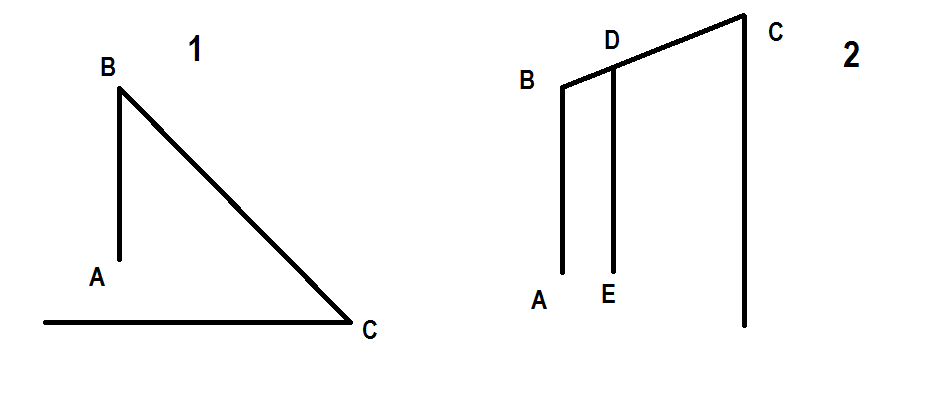
\includegraphics[scale = 0.4]{3Engineering/6Specifications_for_modules/bucket/images/01}
   	    \caption{Side view of beams onto which the bucket is mounted}
   	\end{minipage}
  \end{figure}	
  
  \item The bucket, mounted on the beams, which in turn are mounted on the slats are in point A and move together. CB can rotate around point B. DE is the maximum height of the guiding rails. Position 1: the bucket is lying on the ground and collecting debris. Position 2: the bucket is perpendicular to the ground and can deliver the debris to the goals. The needed ratios can be found from the easily derived formula: %<C = АЕ/(DE - BA).
  \item At the time the above process was completed, the qualification rounds were not far away, and so was decided to temporarily use two servos for shifting and turning the bucket, since the structure of the module would become significantly simpler and would require less time to complete. Were connected two slats in such a way that their uppermost part could move in both directions. After that on one of the ends of the slats were added limiters that depending on their position do not let one of the slats move. This does not prevent the robot from working properly, as we know our alliance before the match and thus in which direction we need to extend the bucket. This means we can adjust the limiters before the match.
    \begin{figure}[h]
  	  \begin{minipage}[h]{1\linewidth}
  	  	  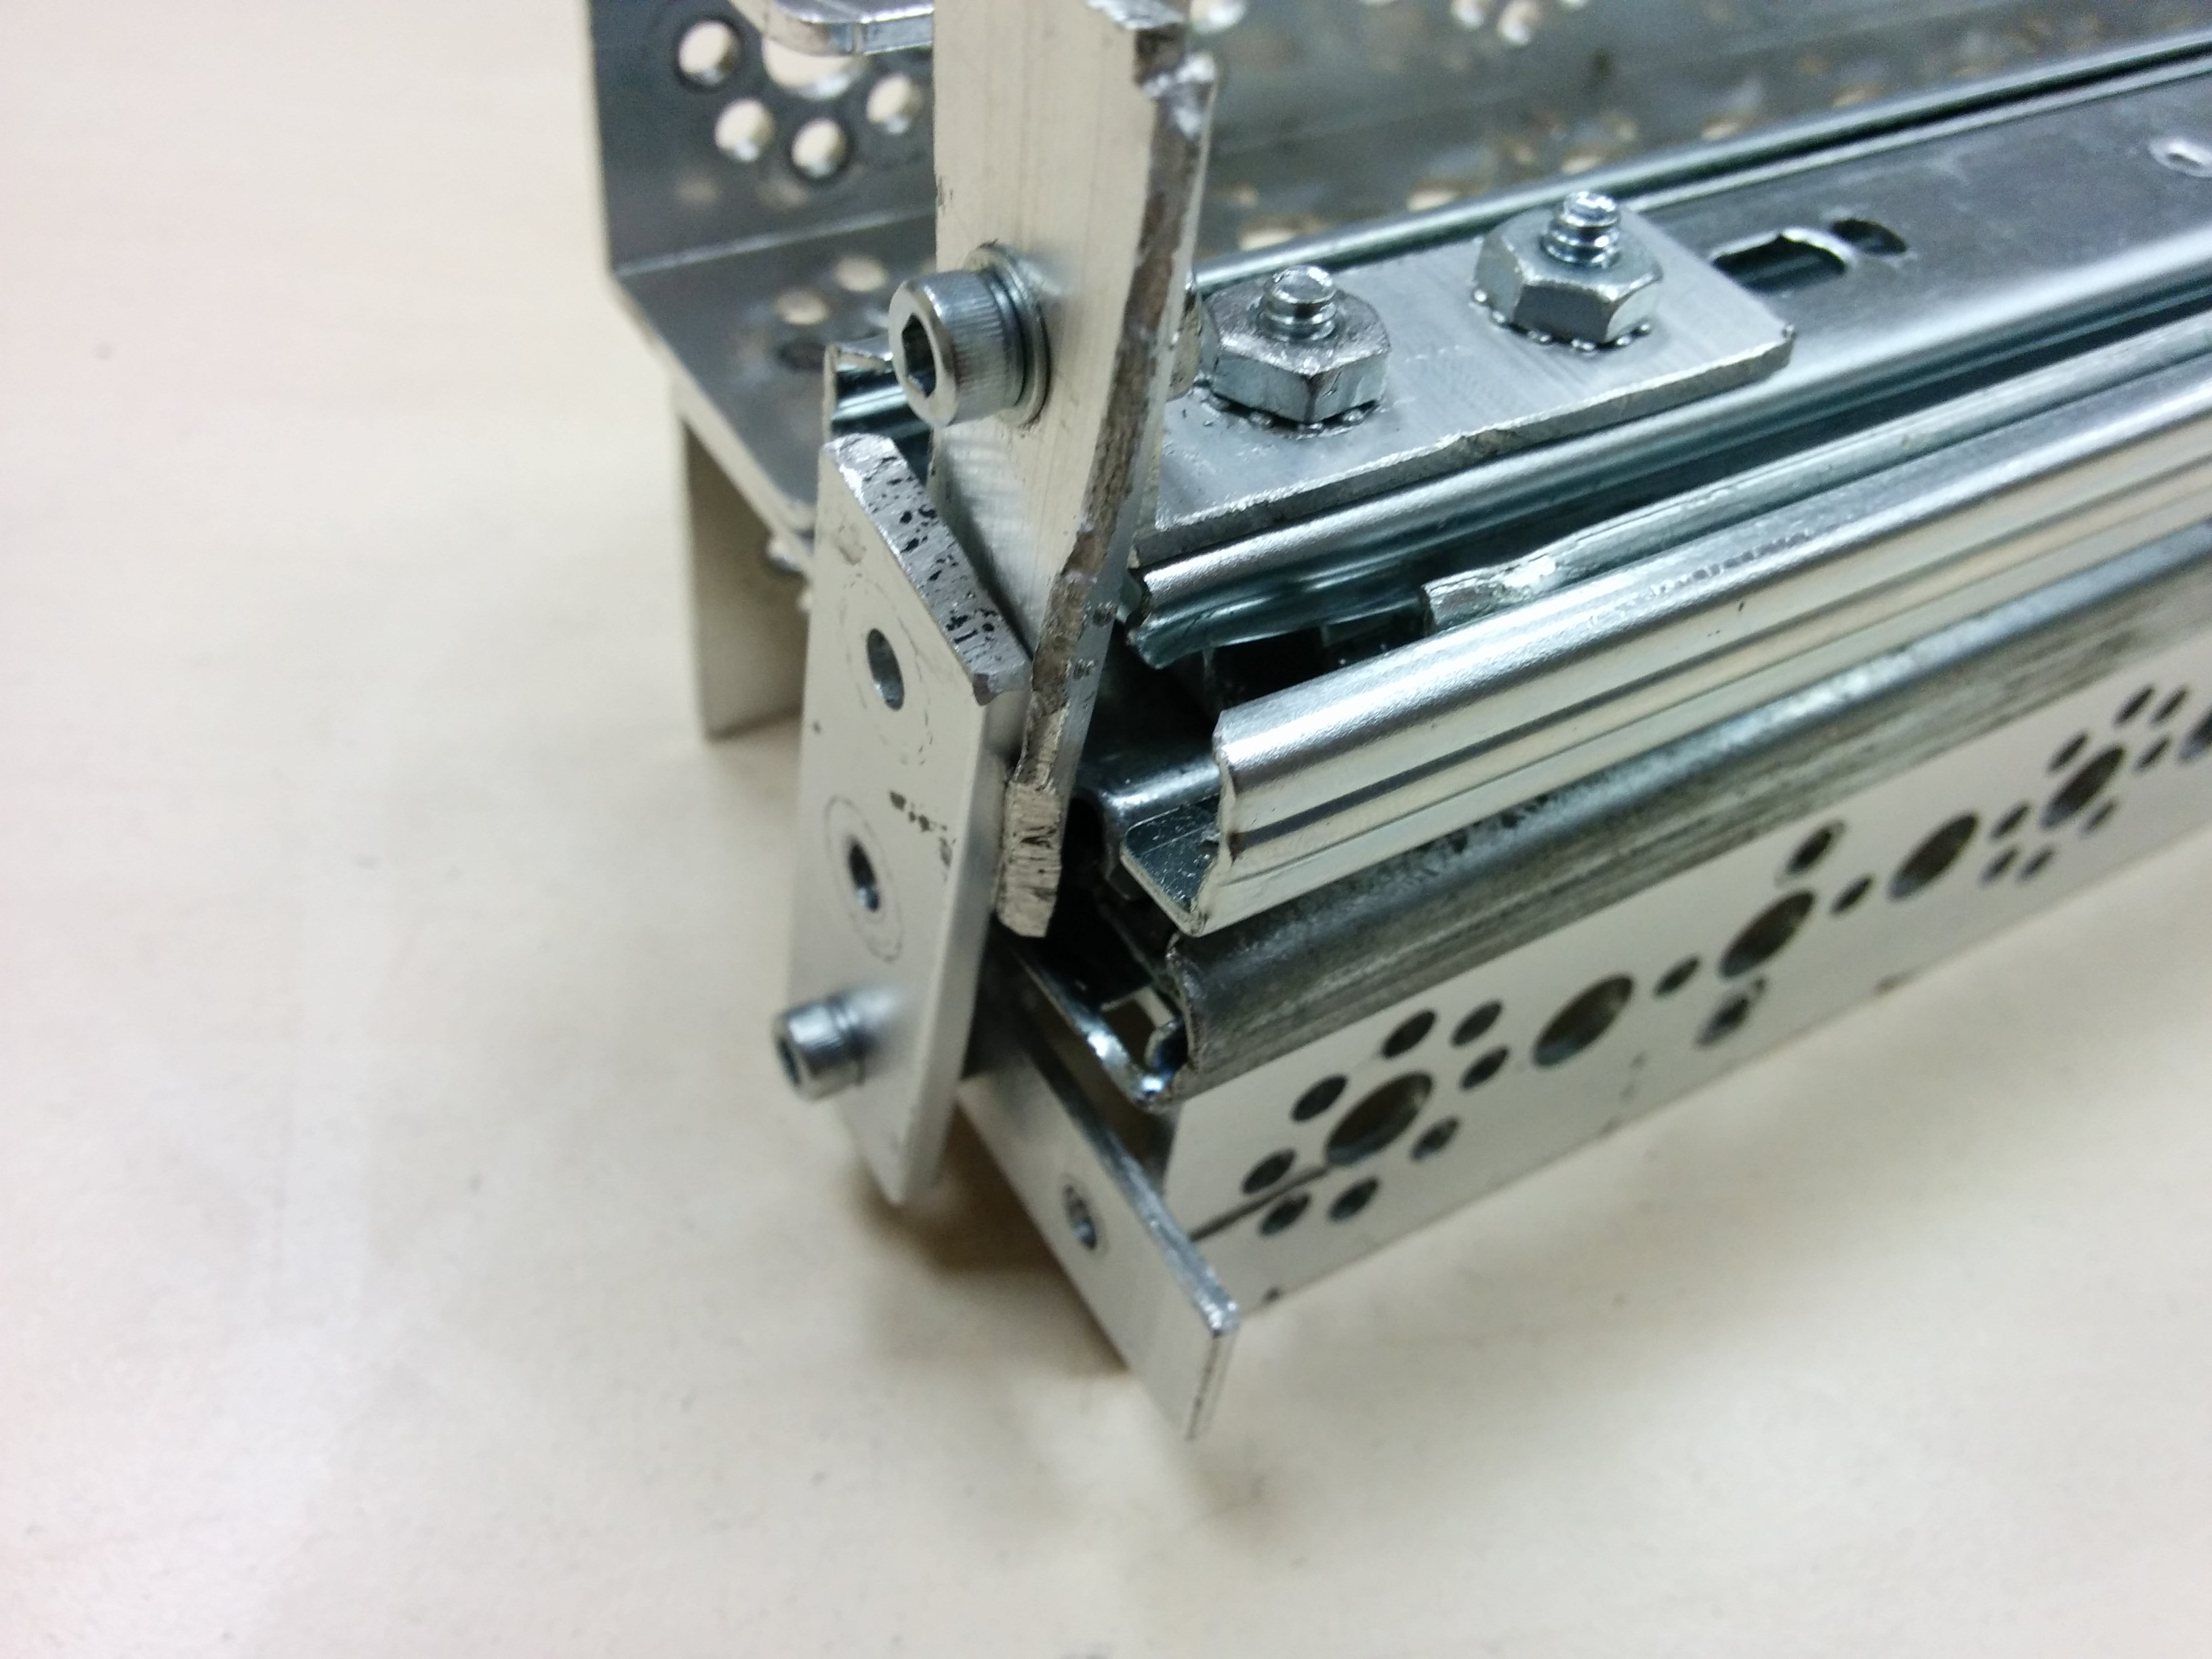
\includegraphics[scale = 0.05]{3Engineering/6Specifications_for_modules/bucket/images/02}
  		  \caption{Structure of limiters}
    	\end{minipage}
    \end{figure}
  (Note: in the figure both limiters are set to the closed position, in which neither slat can move; during the game itself one of the limiters will be set in the open position). 
  \item Then the servo with а reel for the twine moving the slats was fixed on. Blocks were attached to the ends of the fixed beams and wound the twine around them; the ends of the twine are tied to the ends of the slats, which allows them to move as needed. The servo direction of rotation defines the direction of movement of the slats and the bucket. 	
  
  \item After that was come up, tested and made another, less complicated, trapezoidal bucket with the opened part smaller than closed. The construction of the guides on the top of bucket would make debris fall in sequence 2-2-1 from the bottom, that way the scoring goals will hold maximum number of debris.
  \begin{figure}[H]
  	\begin{minipage}[h]{0.31\linewidth}
  		\center{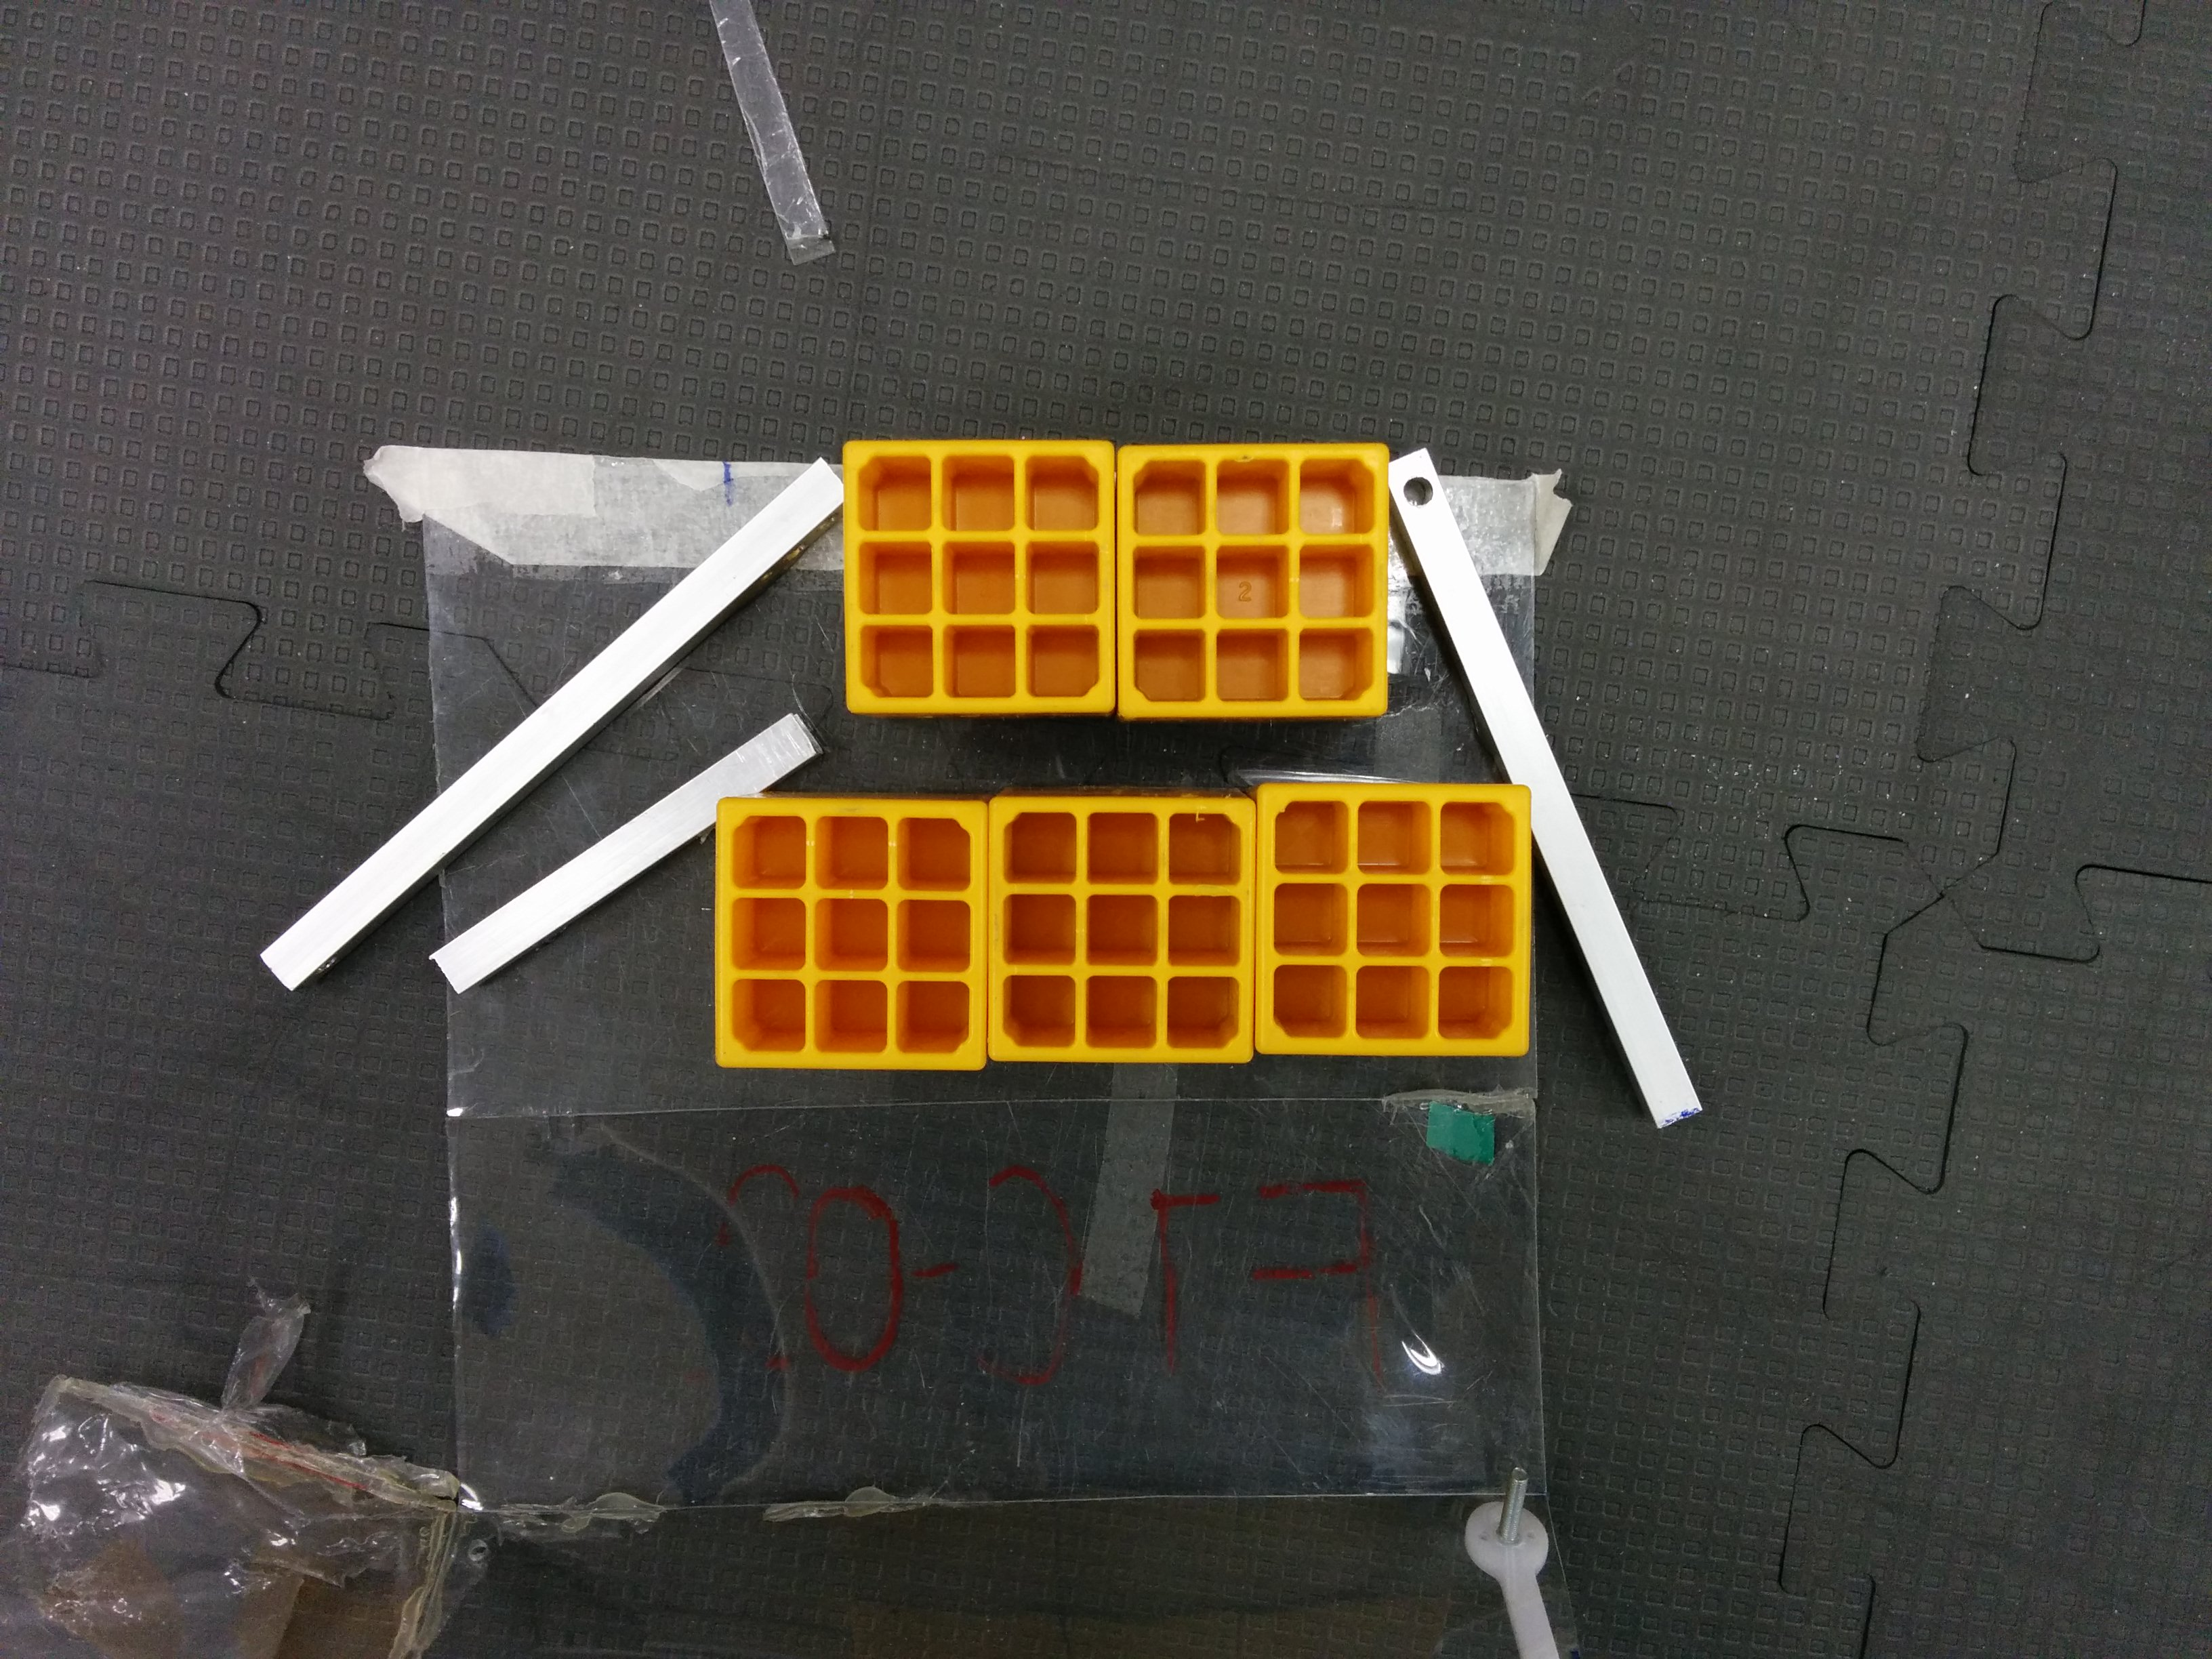
\includegraphics[scale = 0.04]{3Engineering/6Specifications_for_modules/bucket/images/03}}
  		\caption{Structure of guides}
  	\end{minipage}
  	\hfill
  	\begin{minipage}[h]{0.31\linewidth}
  		\center{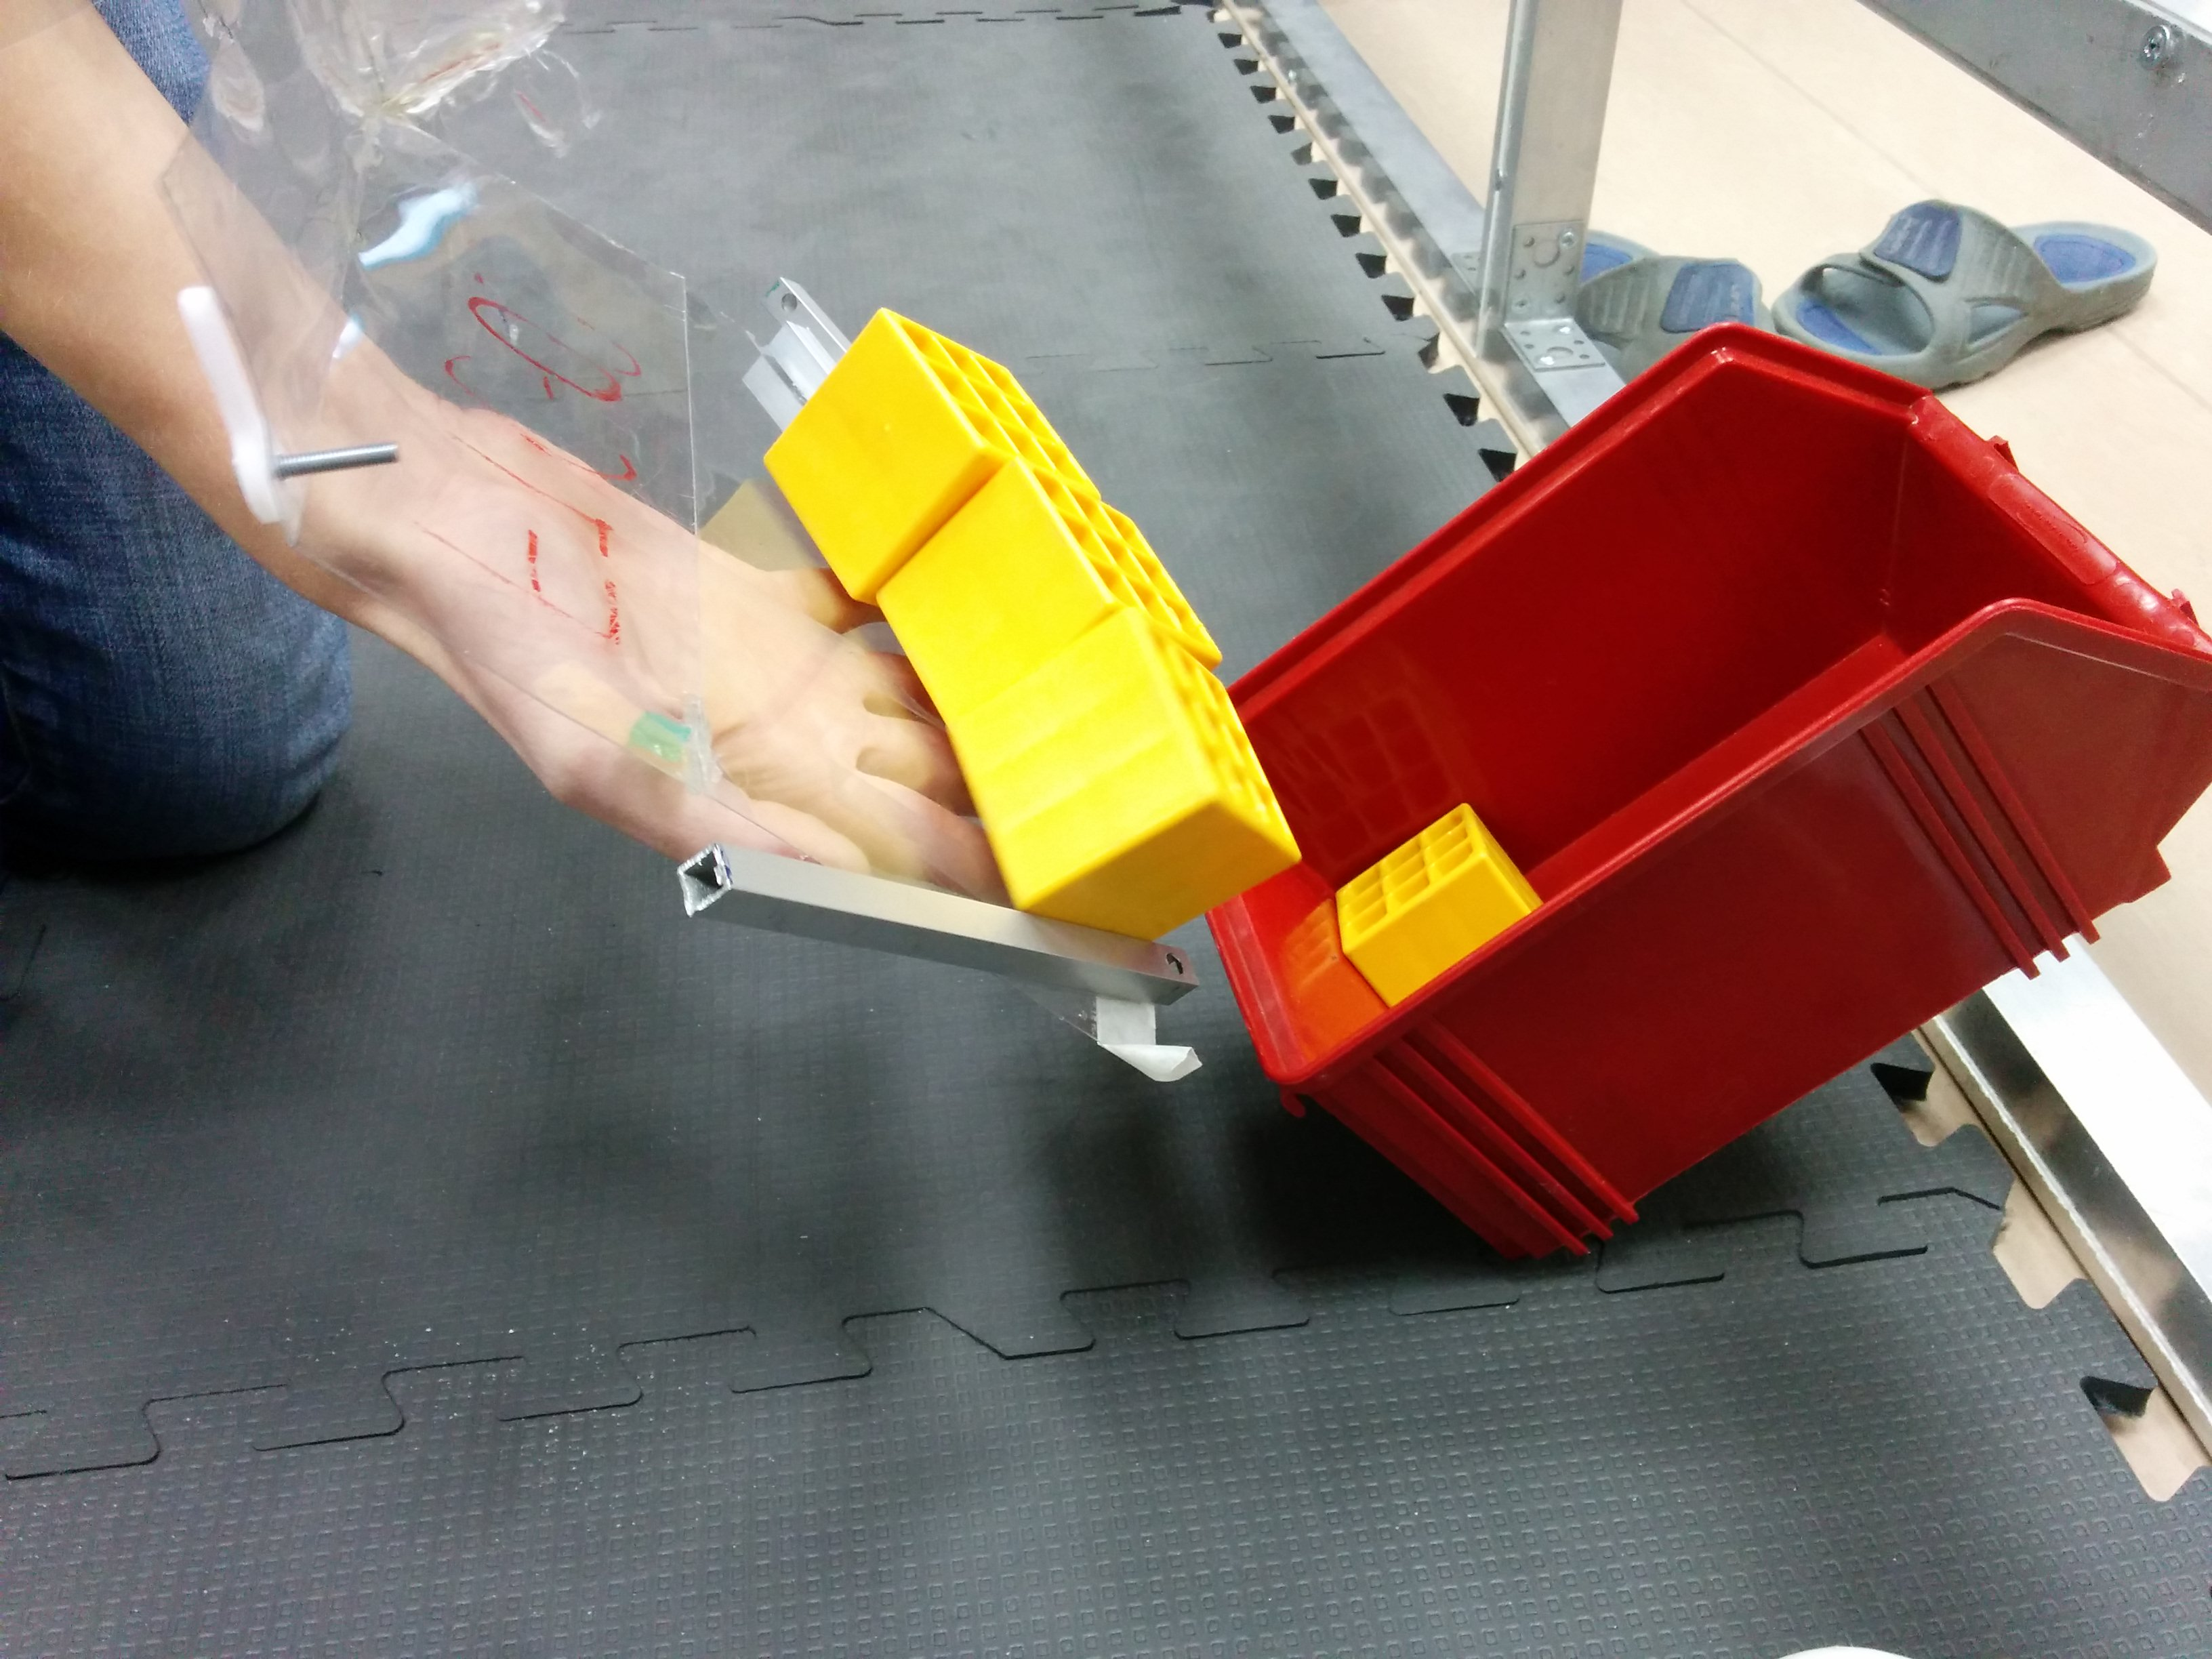
\includegraphics[scale = 0.04]{3Engineering/6Specifications_for_modules/bucket/images/04}}
  		\caption{Process of guides testing}
  	\end{minipage}
  	\hfill
  	\begin{minipage}[h]{0.31\linewidth}
  		\center{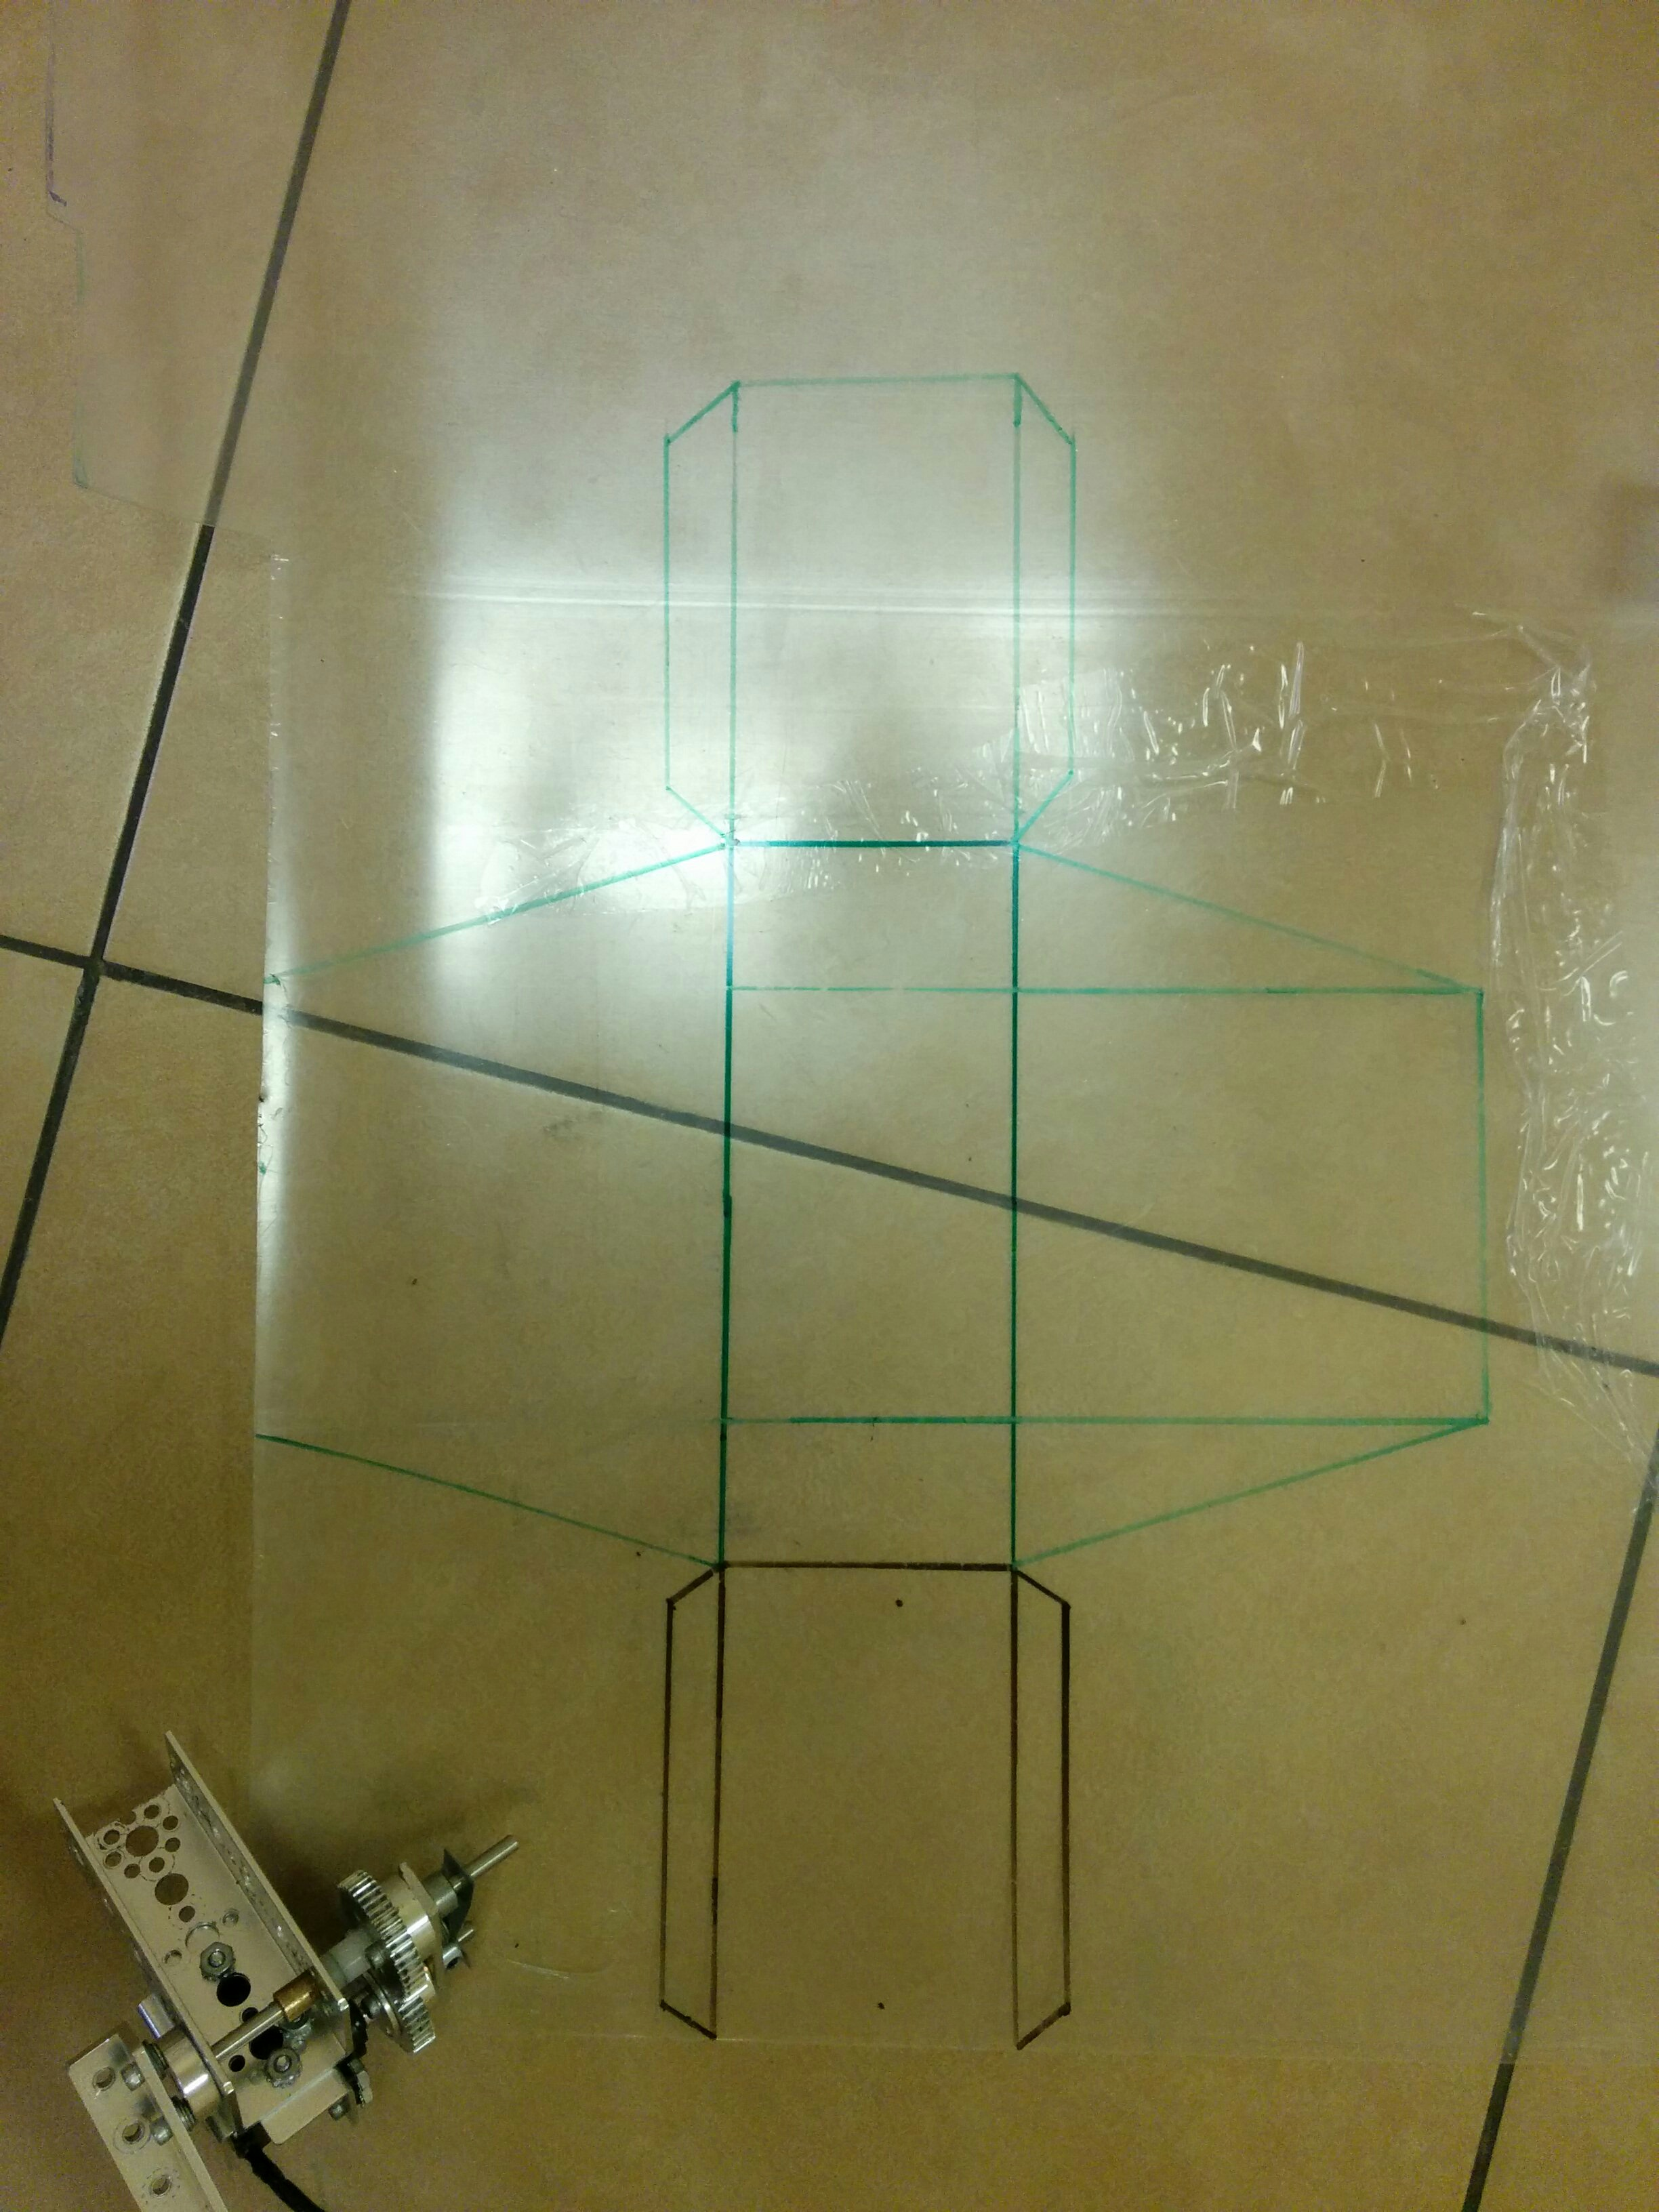
\includegraphics[scale = 0.04]{3Engineering/6Specifications_for_modules/bucket/images/05}}
  		\caption{Marking of bucket}
  	\end{minipage}
  \end{figure}
  Tests showed that guides work well, so was decided to use them in construction of bucket. The pair of front makes debris fall to the scoring goals more accurately, the asymmetric guide slows one debris to make all the debris fall as 2-2-1, not 2-3.
 
  \item After that was stretched the line to move the slats. Servos for moving the slats and turning the bucket were placed on the slats.
  \begin{figure}[H]
  	\begin{minipage}[h]{0.47\linewidth}
  		\center{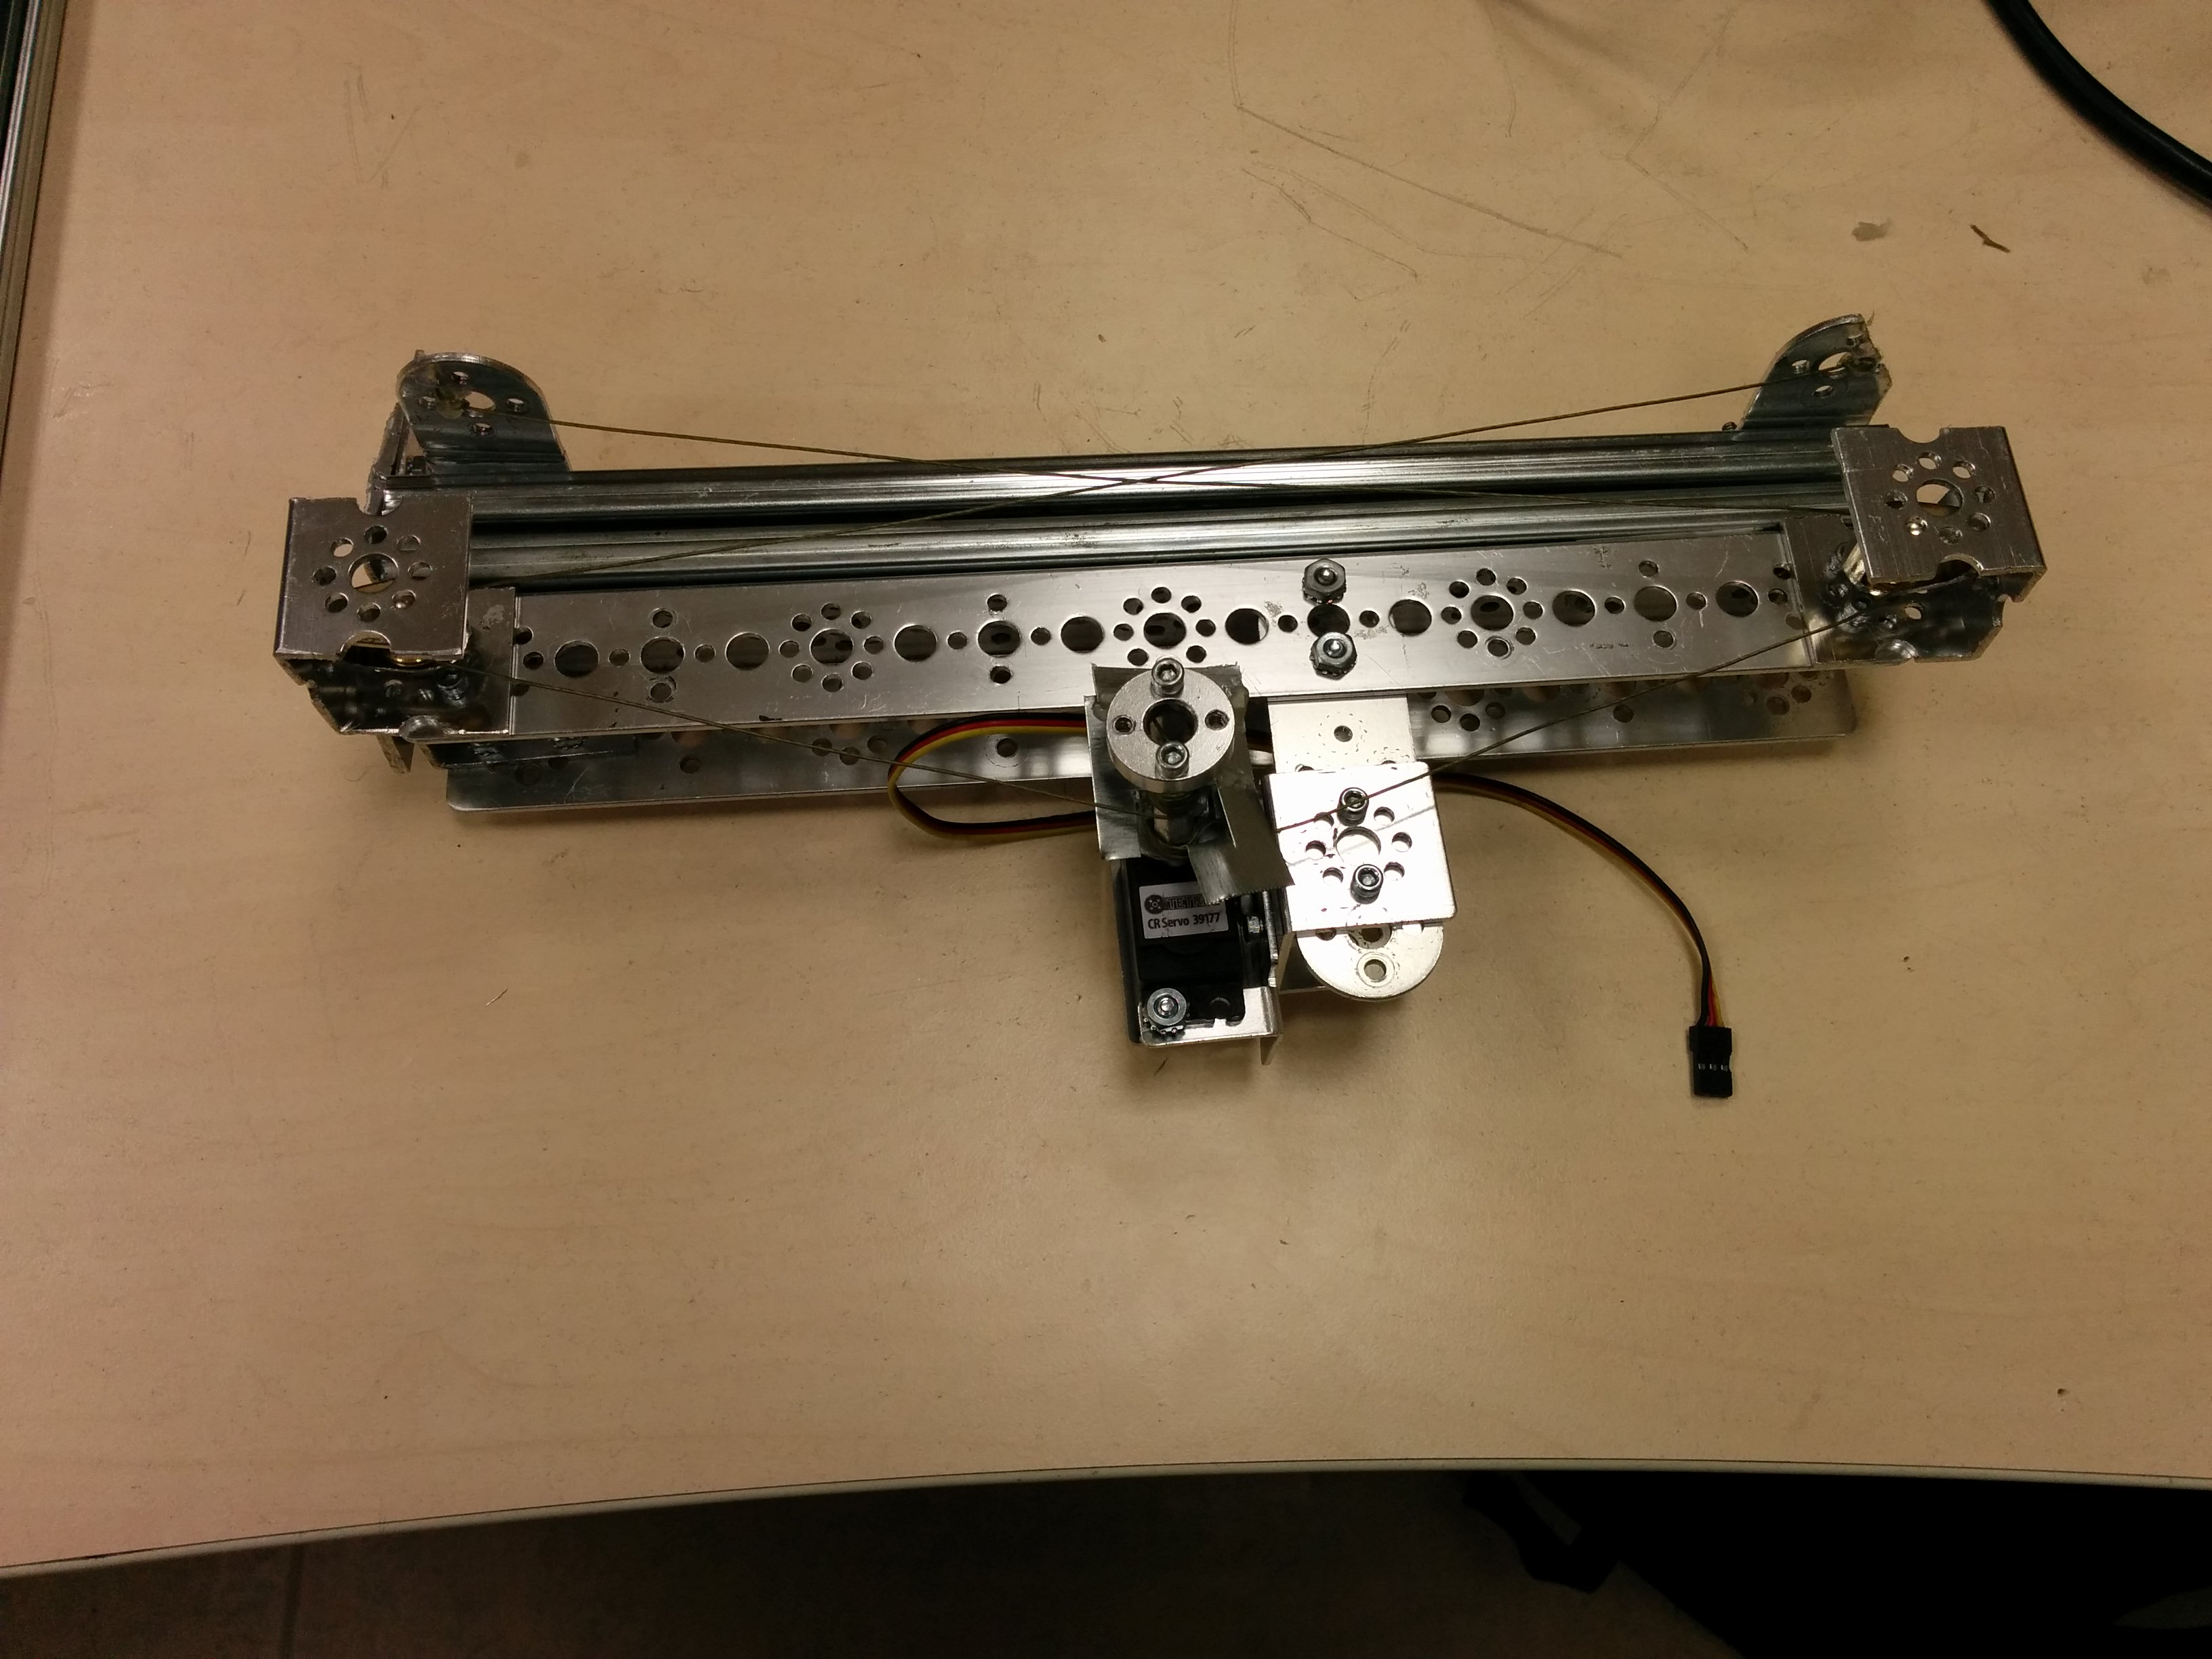
\includegraphics[scale = 0.05]{3Engineering/6Specifications_for_modules/bucket/images/06}}
  		\caption{Construction of line and pulling it servo}
  	\end{minipage}
  	\hfill
  	\begin{minipage}[h]{0.47\linewidth}
  		\center{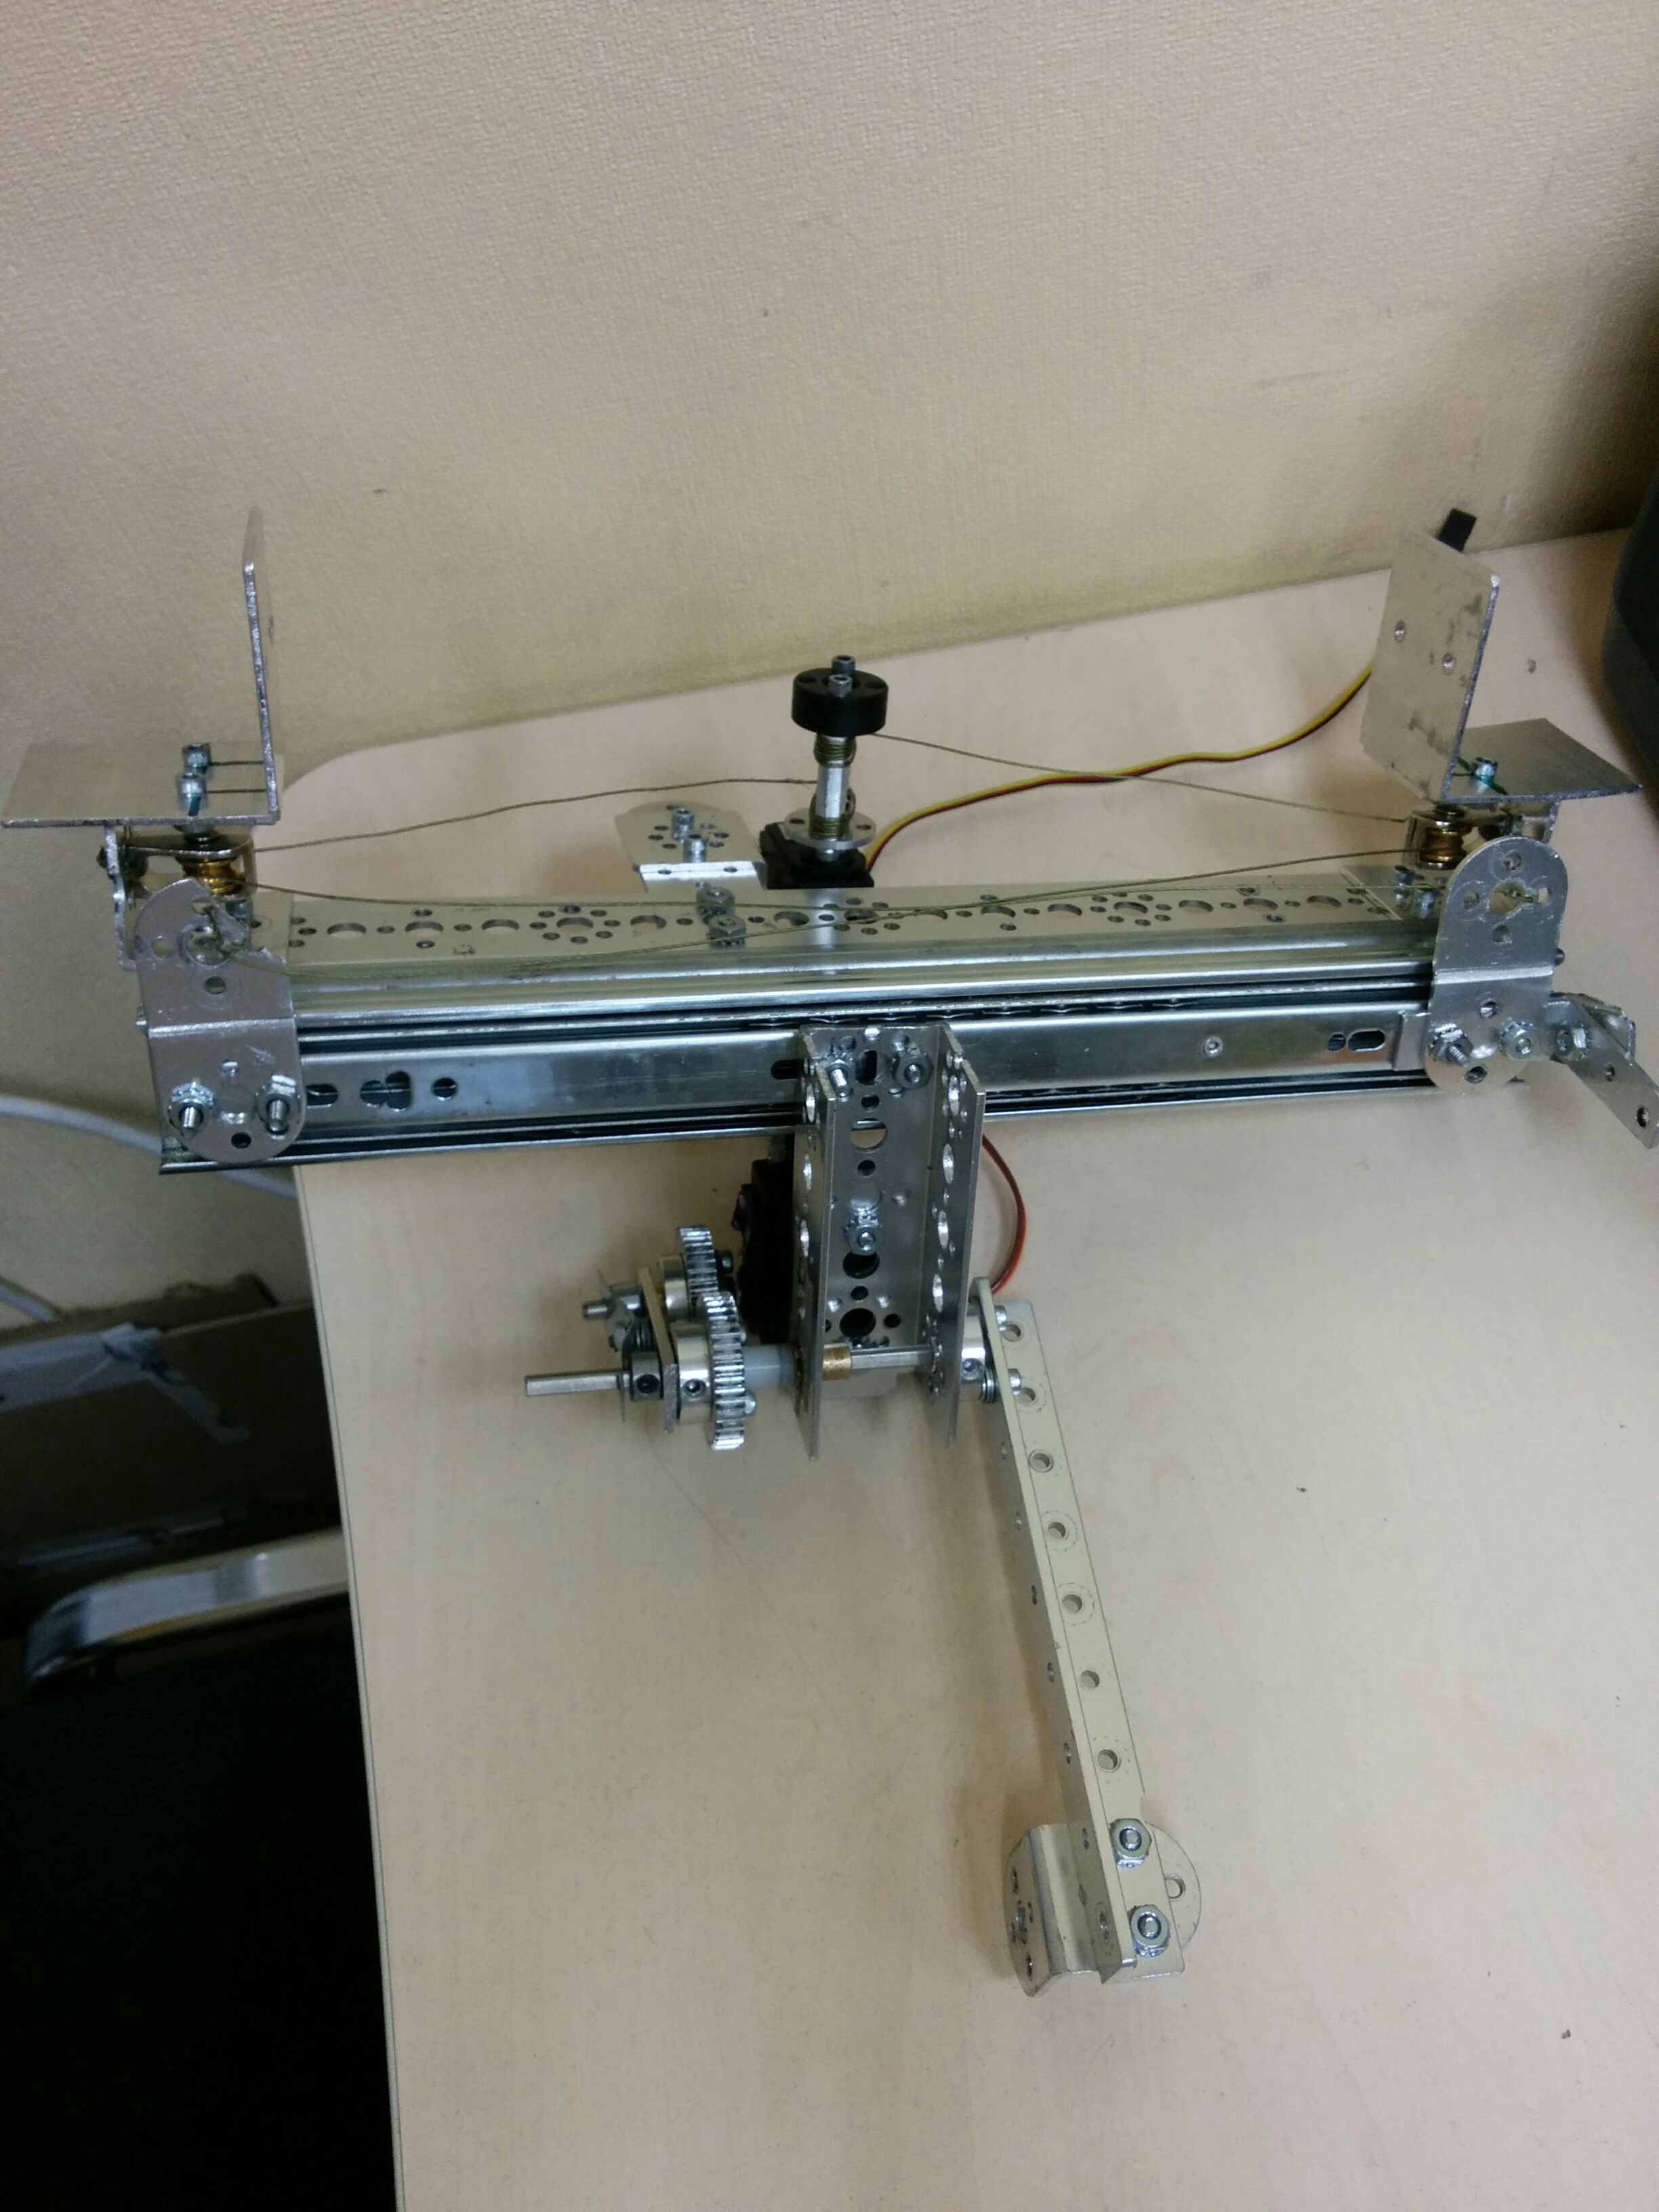
\includegraphics[scale = 0.05]{3Engineering/6Specifications_for_modules/bucket/images/07}}
  		\caption{Final construction of the slats}
  	\end{minipage}
  \end{figure}
  
  \item Next done part of module is closing mechanism. The difficulty in it is that axis of servo has to be as close as possible to the front-top edge of bucket.
  
  \begin{figure}[H]
  	\begin{minipage}[h]{1\linewidth}
  		\center{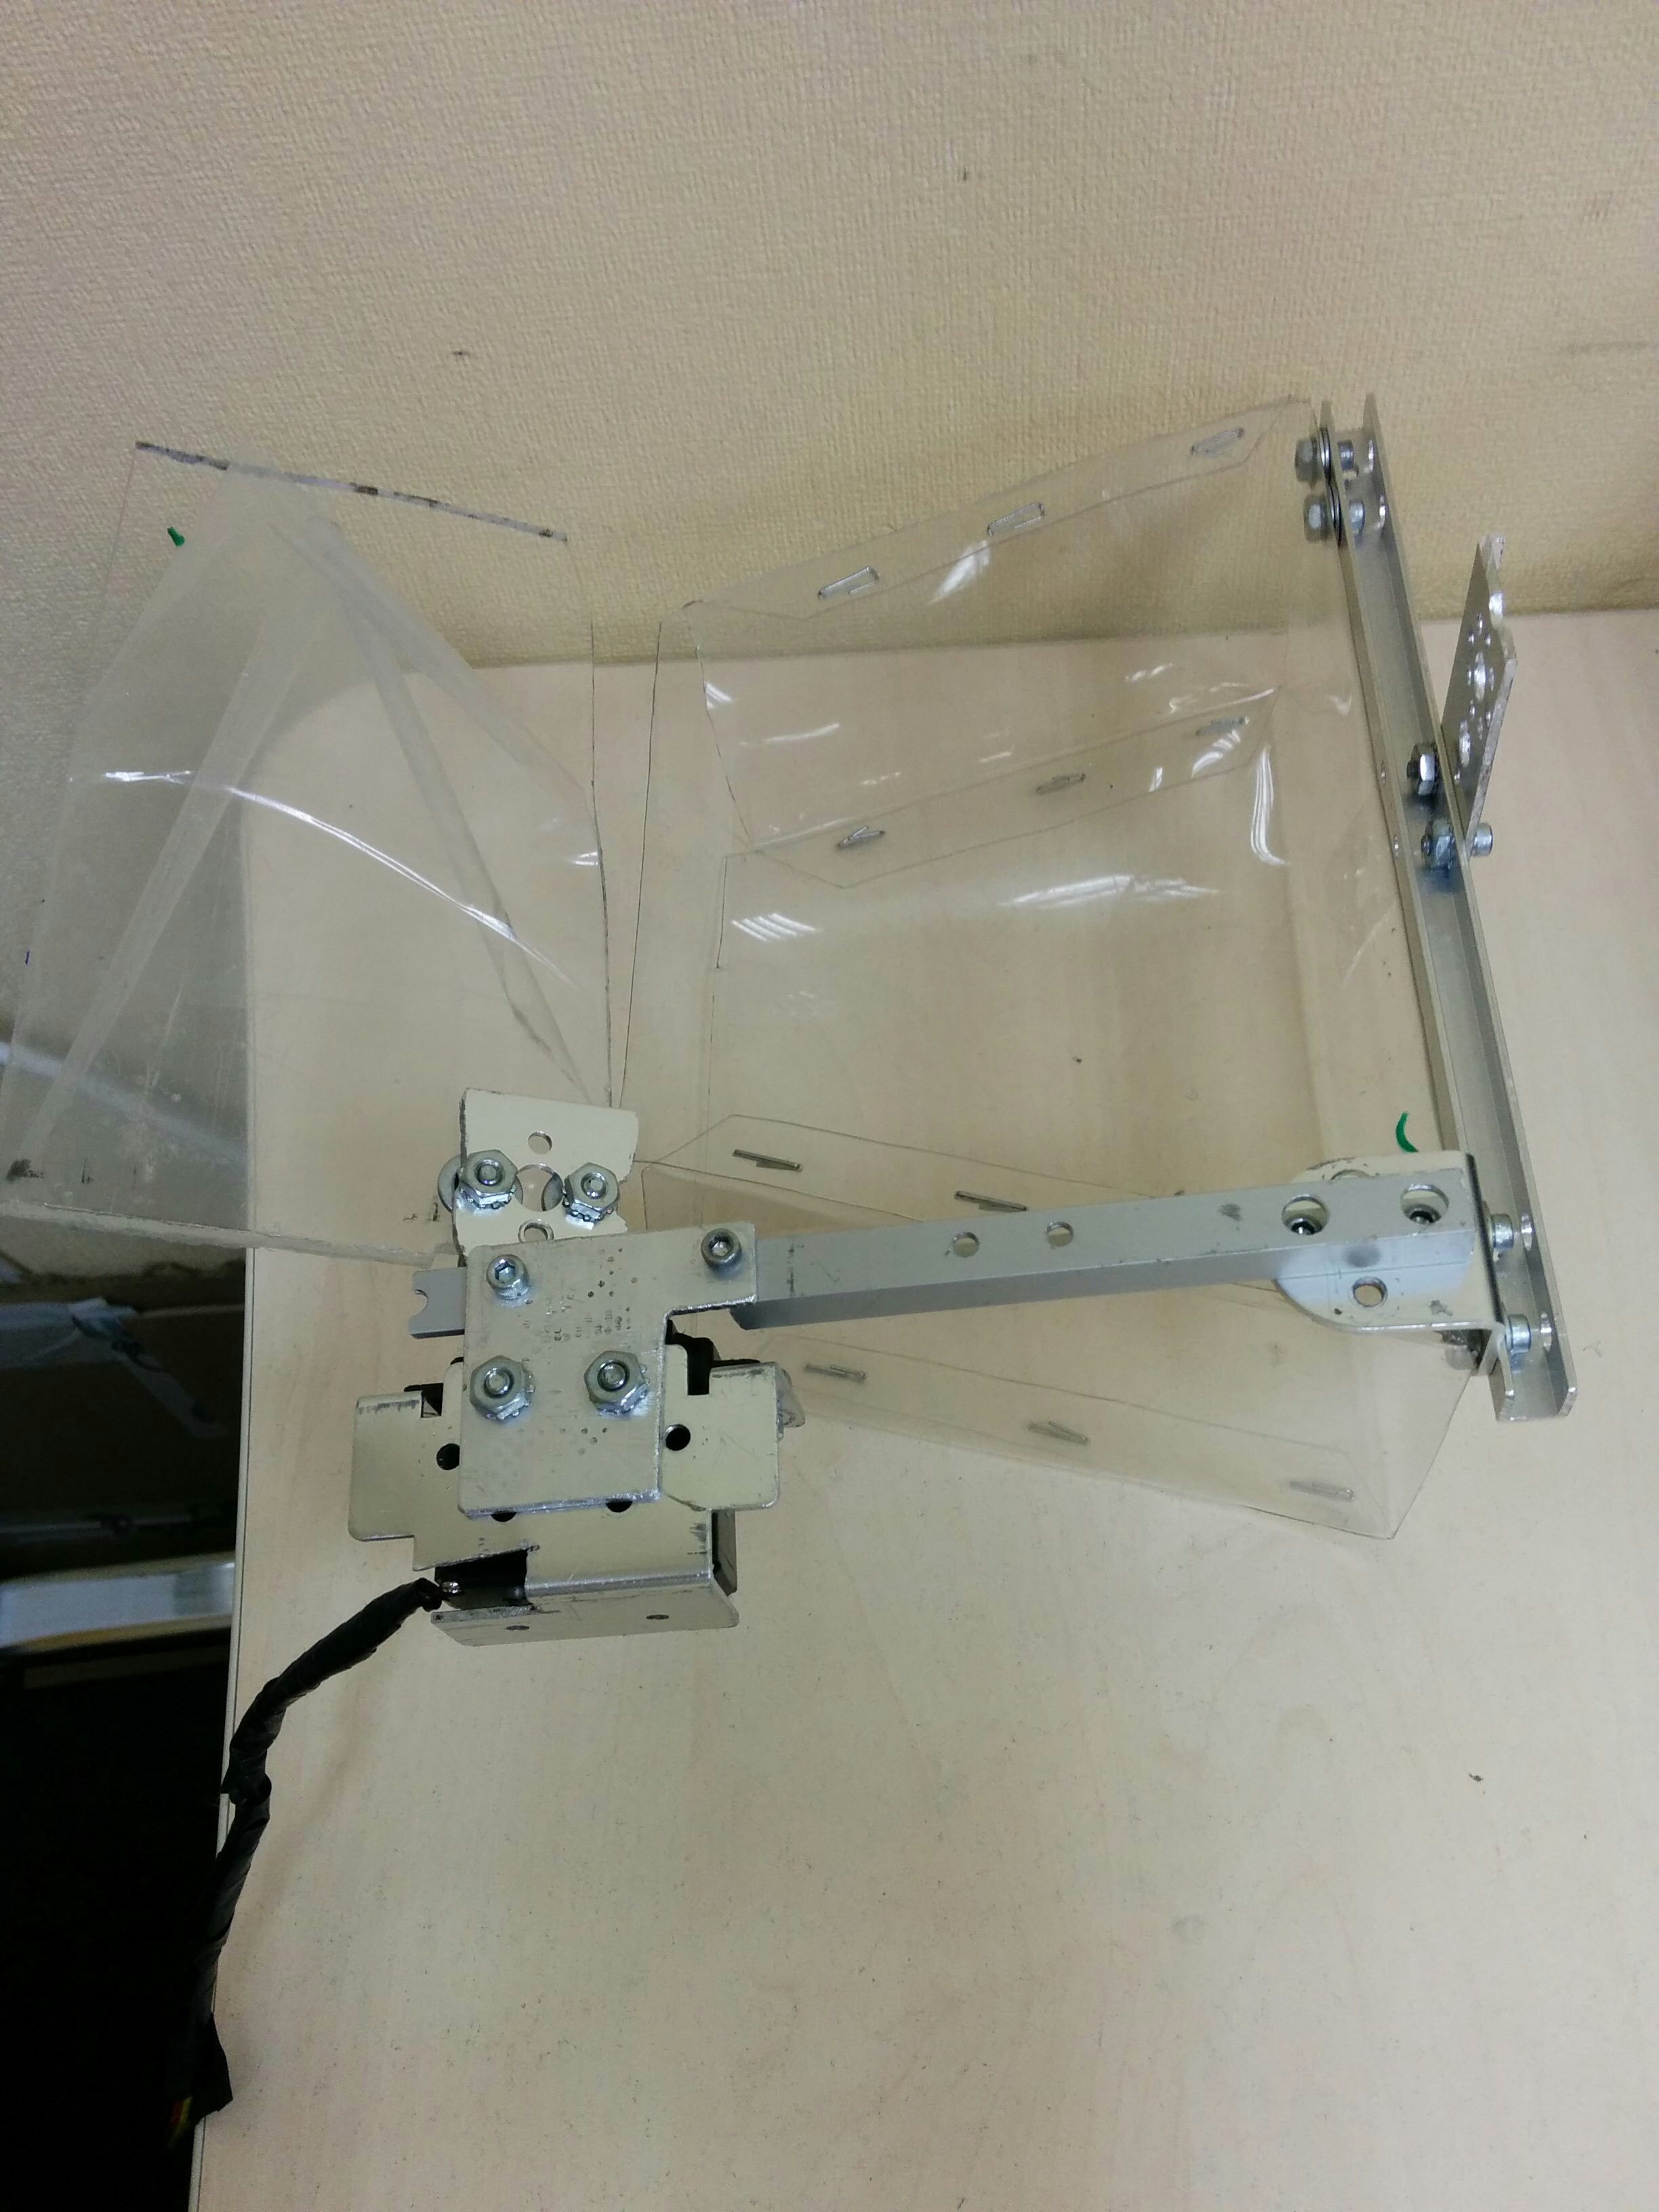
\includegraphics[scale = 0.05]{3Engineering/6Specifications_for_modules/bucket/images/08}}
  		\caption{Final construction of the bucket with closing mechanism}
  	\end{minipage}
  \end{figure}
  
  \item After that bucket was installed on bracings on the slats. Then all the module was mounted on the lifting mechanism. It was done in the way to make the bucket turning axis as low as possible. It would make the volume, used by bucket less, because with that place of the bucket it was necessary to turn it while lifting because otherwise bucket intersected with other parts of robot while lifting. So the lower axis made the radius of bucket turning less and reduced the capacity on the servo by shortening the shoulder of buckets weight.
  By the time it was done, the first competitions had almost started so the slats weren't mounted on the lift because of time troubles.
  
  \item After the end of competitions slats were replaced by longer ones (40 cm instead of 35) to make bucket shifting completely out of robot theoretically possible. Also the shifting servo was changed to faster and more powerful servo in order to make bucket shifting faster and more reliability. Then possible work process of bucket was estimated and it turned that fast lifting was impossible. It was so because the bucket was to be turned in case not to intersect with other parts of robot to be lifted. And generally bucket was close to catch parts of robot while moving from front of robot to its end during the lifting. To solve these problems was decided to place the bucket into end of the robot above two beams. It would make lifting easier because bucket would move inside robots projection much less time than before, also it is easier to transport debris throw the robot than to transport the bucket.
  \item Then the slats were mounted on this lift in the way to place bucket in the end of robot. The next problem was not much space so the beam, on which the bucket was mounted intersected with lifts slats while shifting. So the mount of the bucket was changed. 
  With that construction servo was turning with the bucket. It made the non-intersection beam possible. After that bucket was mounted on the sift mechanism without any intersections, so the problem was solved.
  
 \begin{figure}[H]
  \begin{minipage}[h]{0.49\linewidth}
  	\center{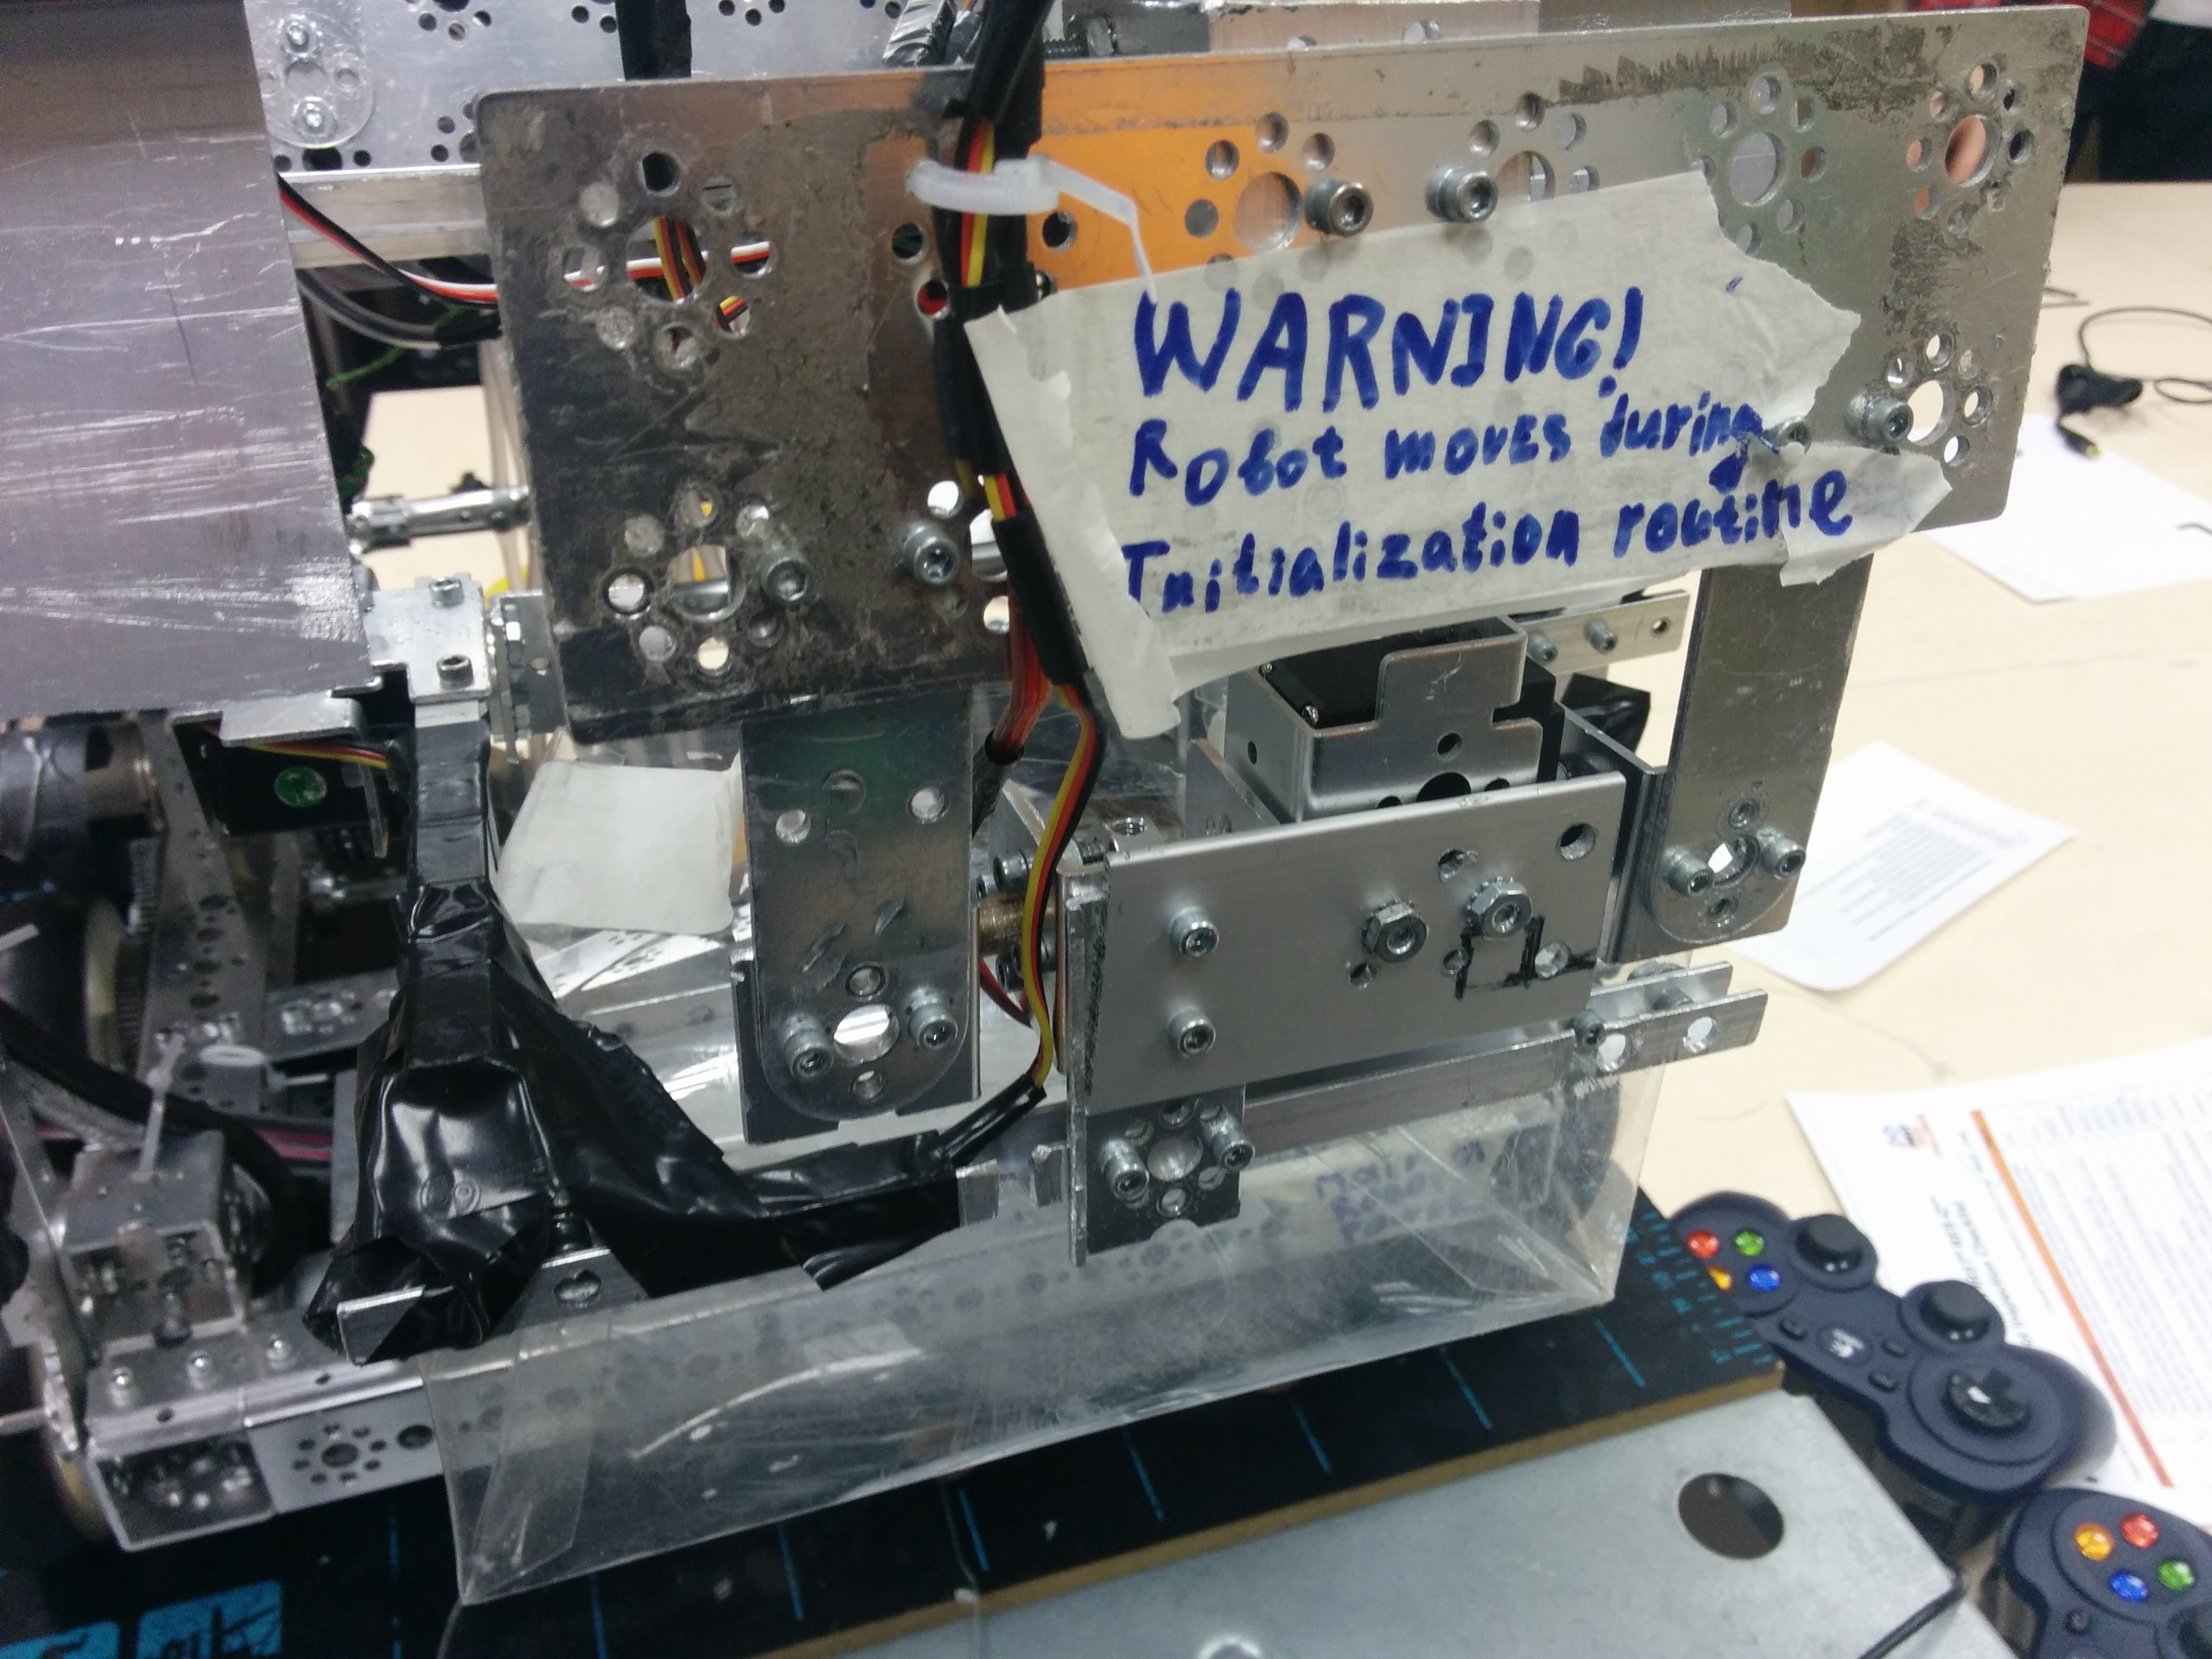
\includegraphics[scale=0.05]{3Engineering/6Specifications_for_modules/bucket/images/09}}
  	\caption{Construction of bucket}
  \end{minipage}
  \begin{minipage}[h]{0.49\linewidth}
  	\center{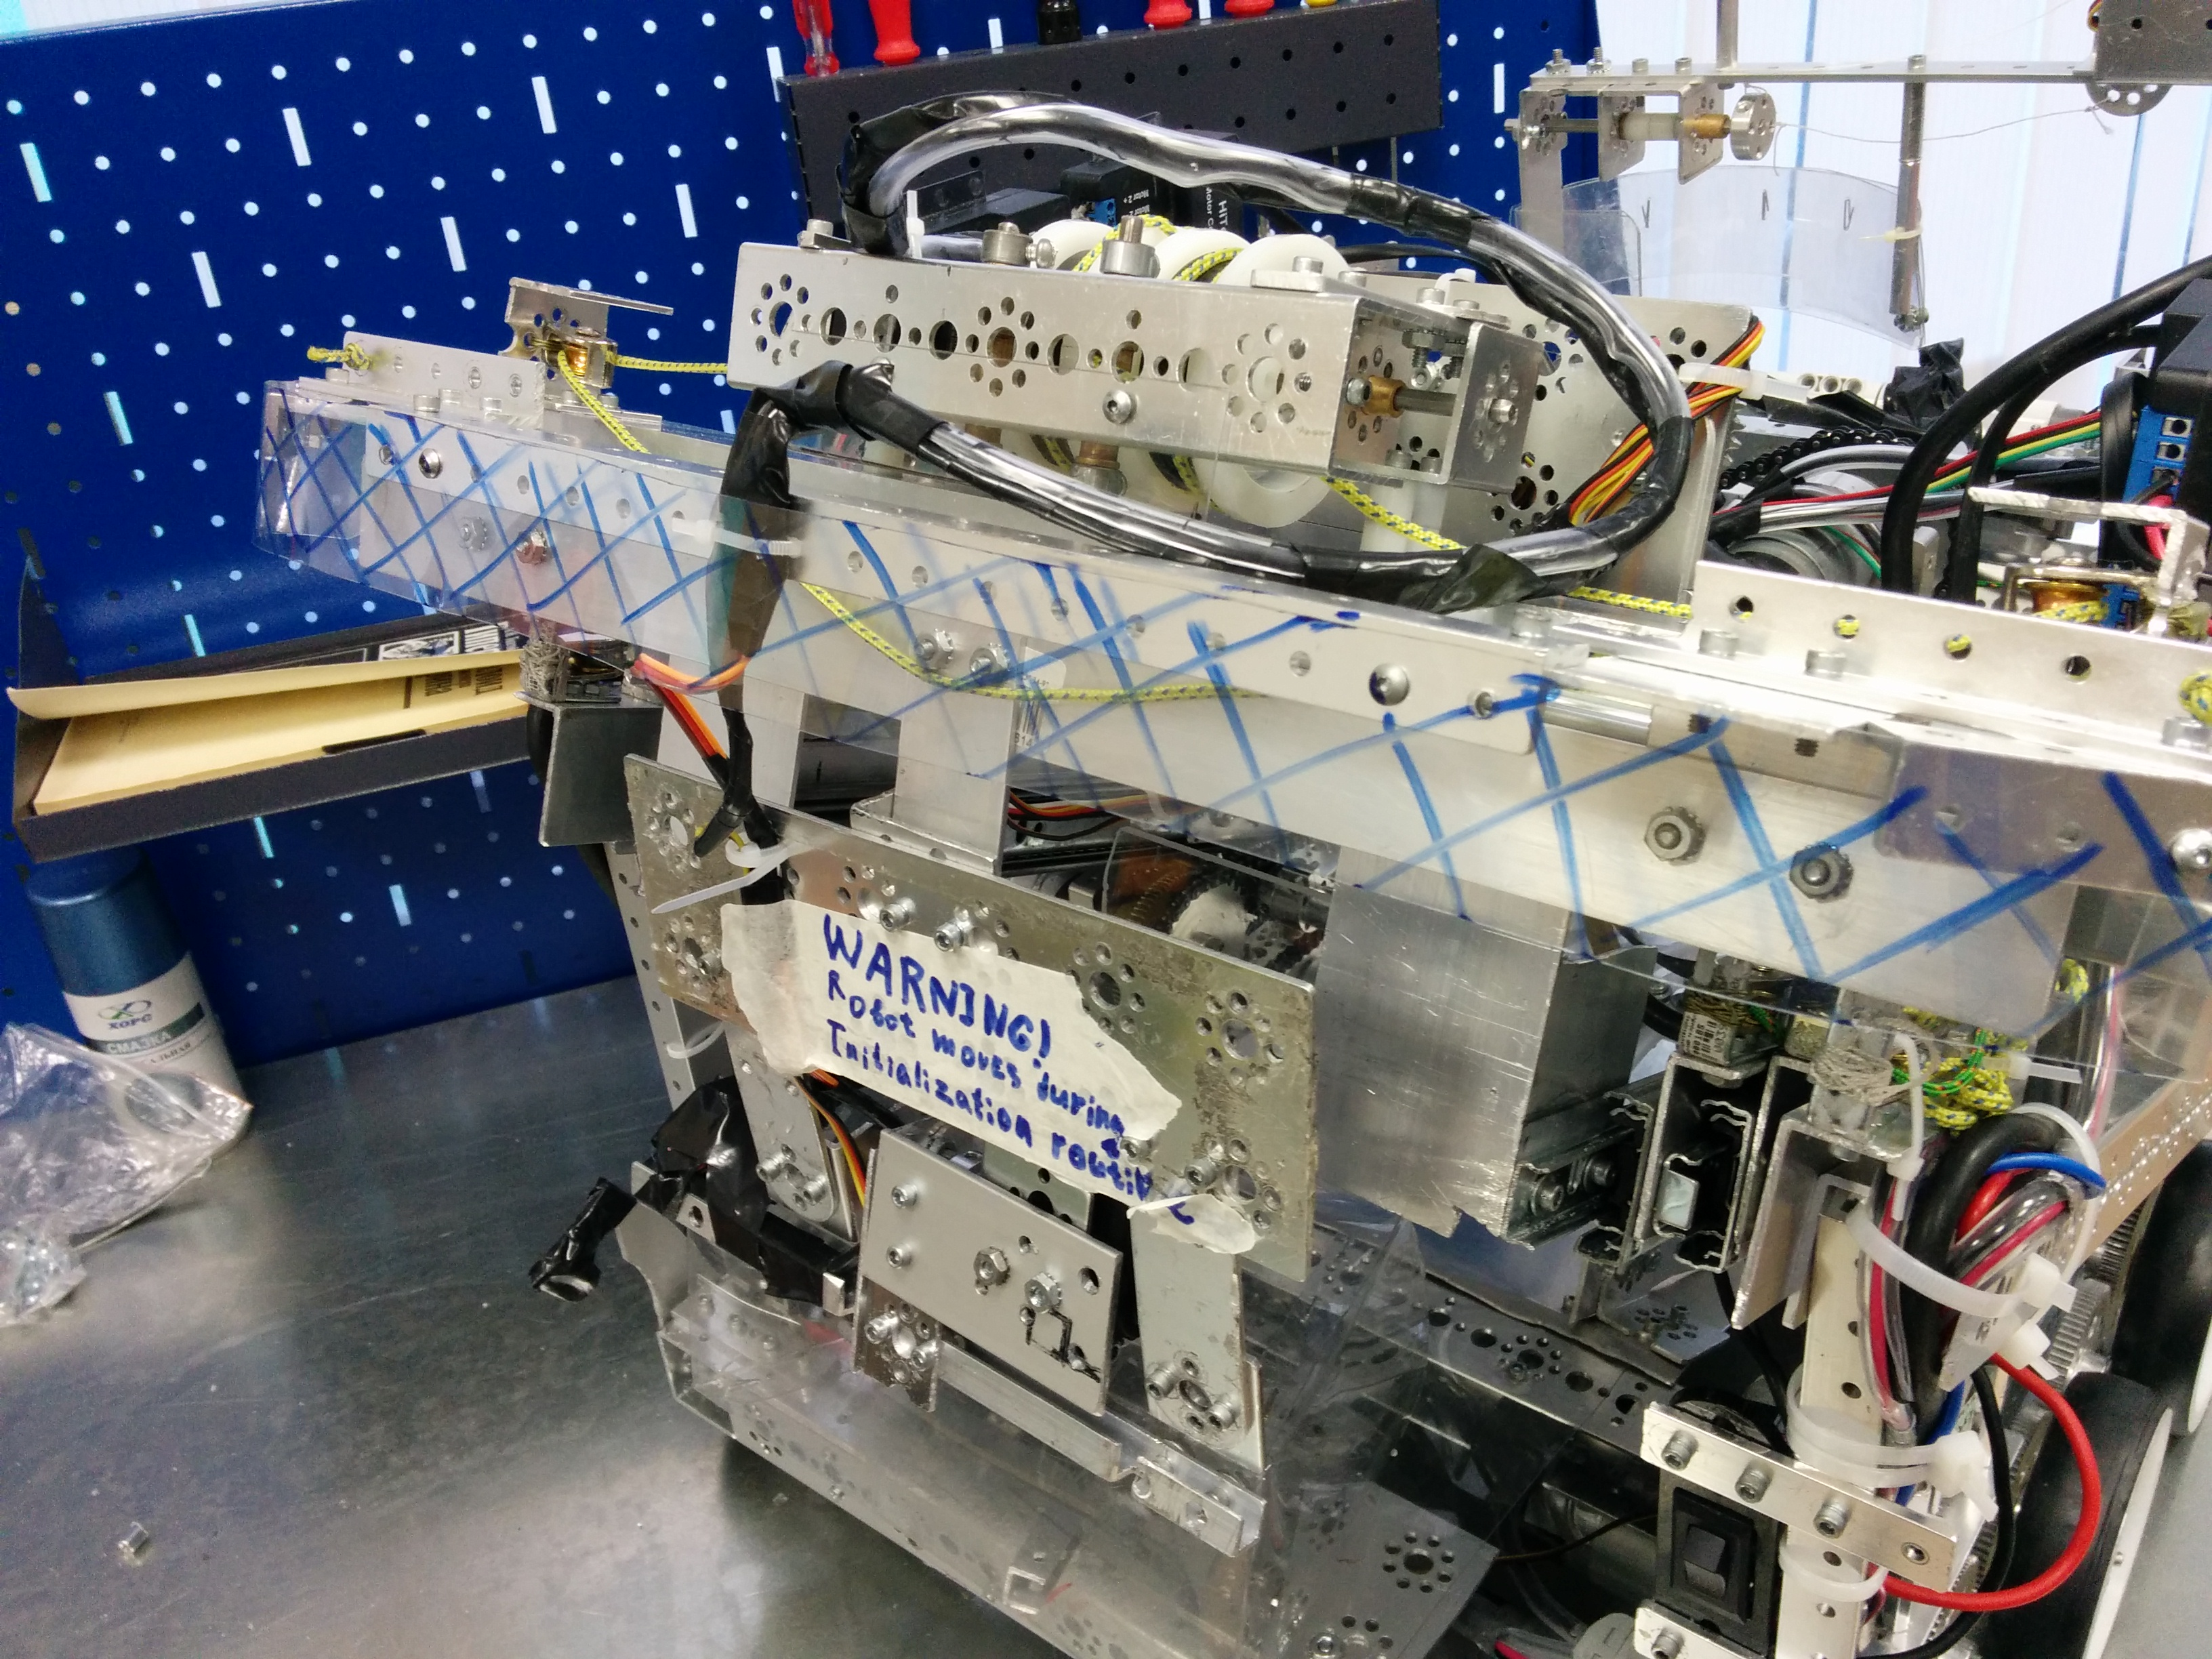
\includegraphics[scale = 0.05]{3Engineering/6Specifications_for_modules/bucket/images/10}}
  	\caption{The bucket mounted on robot}
  \end{minipage}
 \end{figure}
  
  \item The next step was testing bucket and the whole robot. In the process of it was found two problems: the closing mechanism was able to work only when the bucked was a bit lifted and bucket couldn't hold 5 cubes, caught by grab mechanism. First problem was solved by cutting sides of partition, closing bucket. The second problem weren't solved by adding guides to move first cube sideways (grab couldn't move the cube so). Because of it was decided to change the shape of bucket. 
  
  \item After that the new shape was devised. 
  
 \begin{figure}[H]
  \begin{minipage}[h]{0.49\linewidth}
  	\center{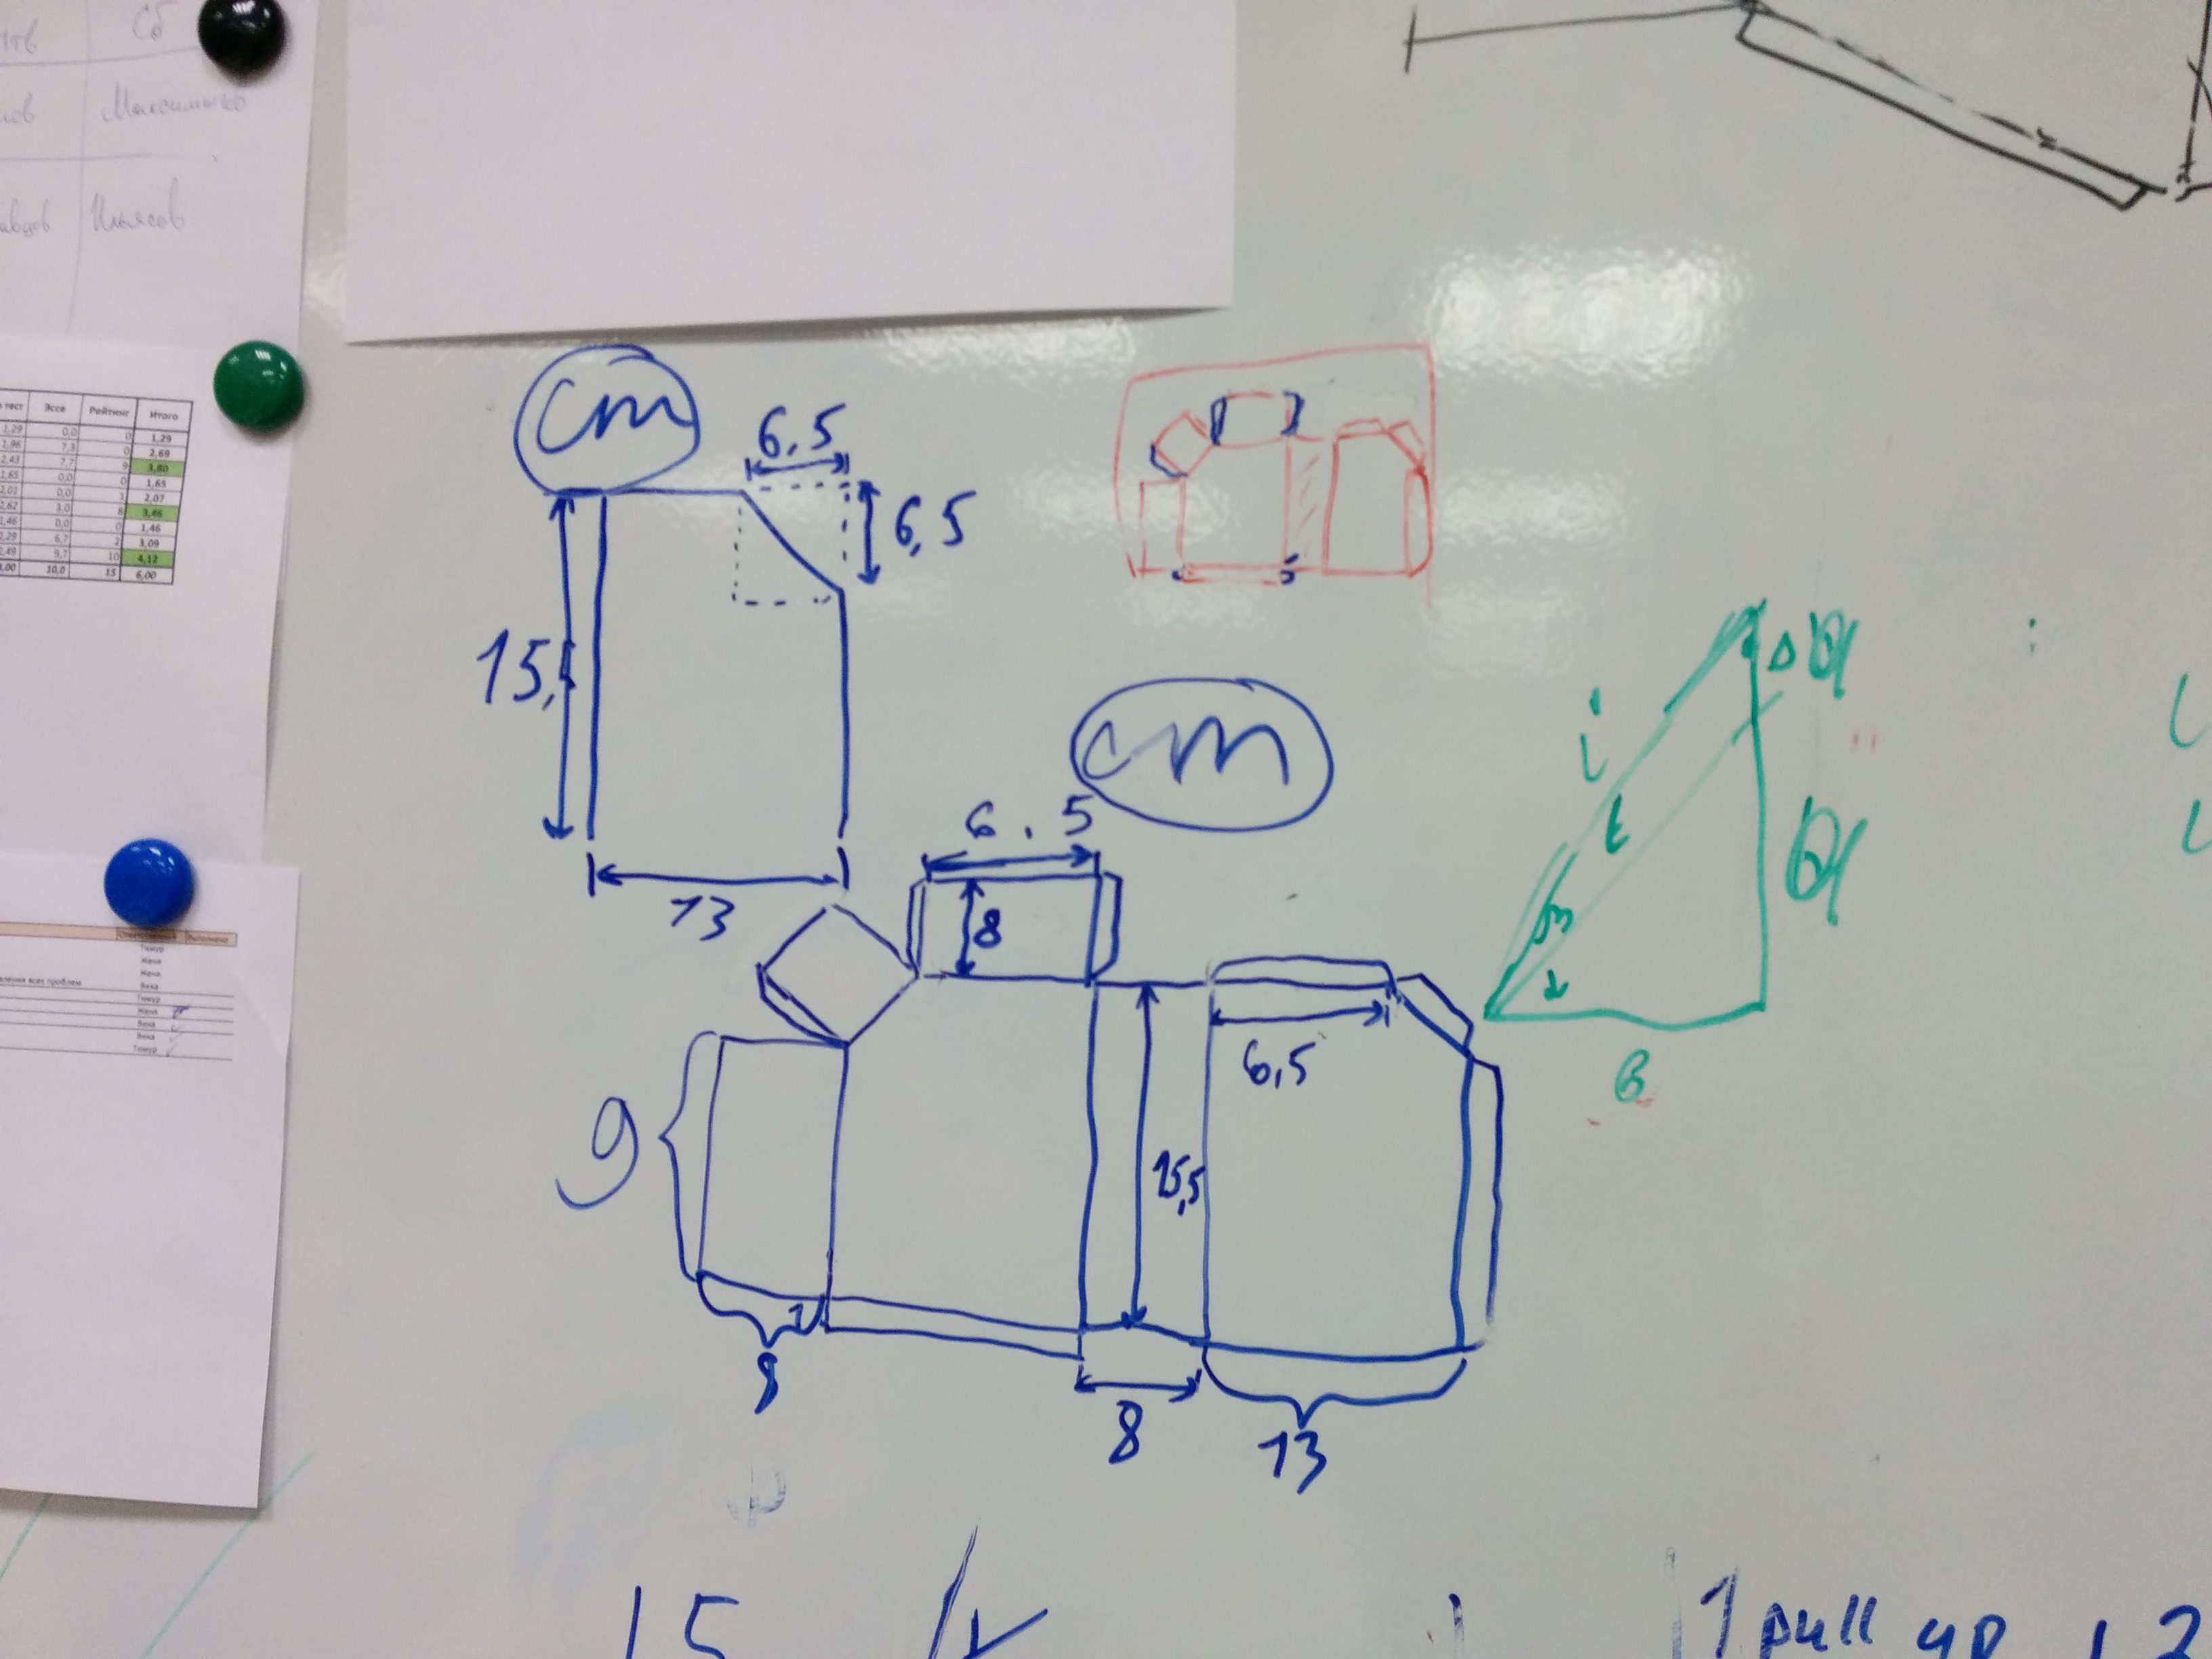
\includegraphics[scale = 0.05]{3Engineering/6Specifications_for_modules/bucket/images/11}}
  	\caption{Shape and scan of the bucket}
  \end{minipage} 
  \begin{minipage}[h]{0.49\linewidth}
  	\center{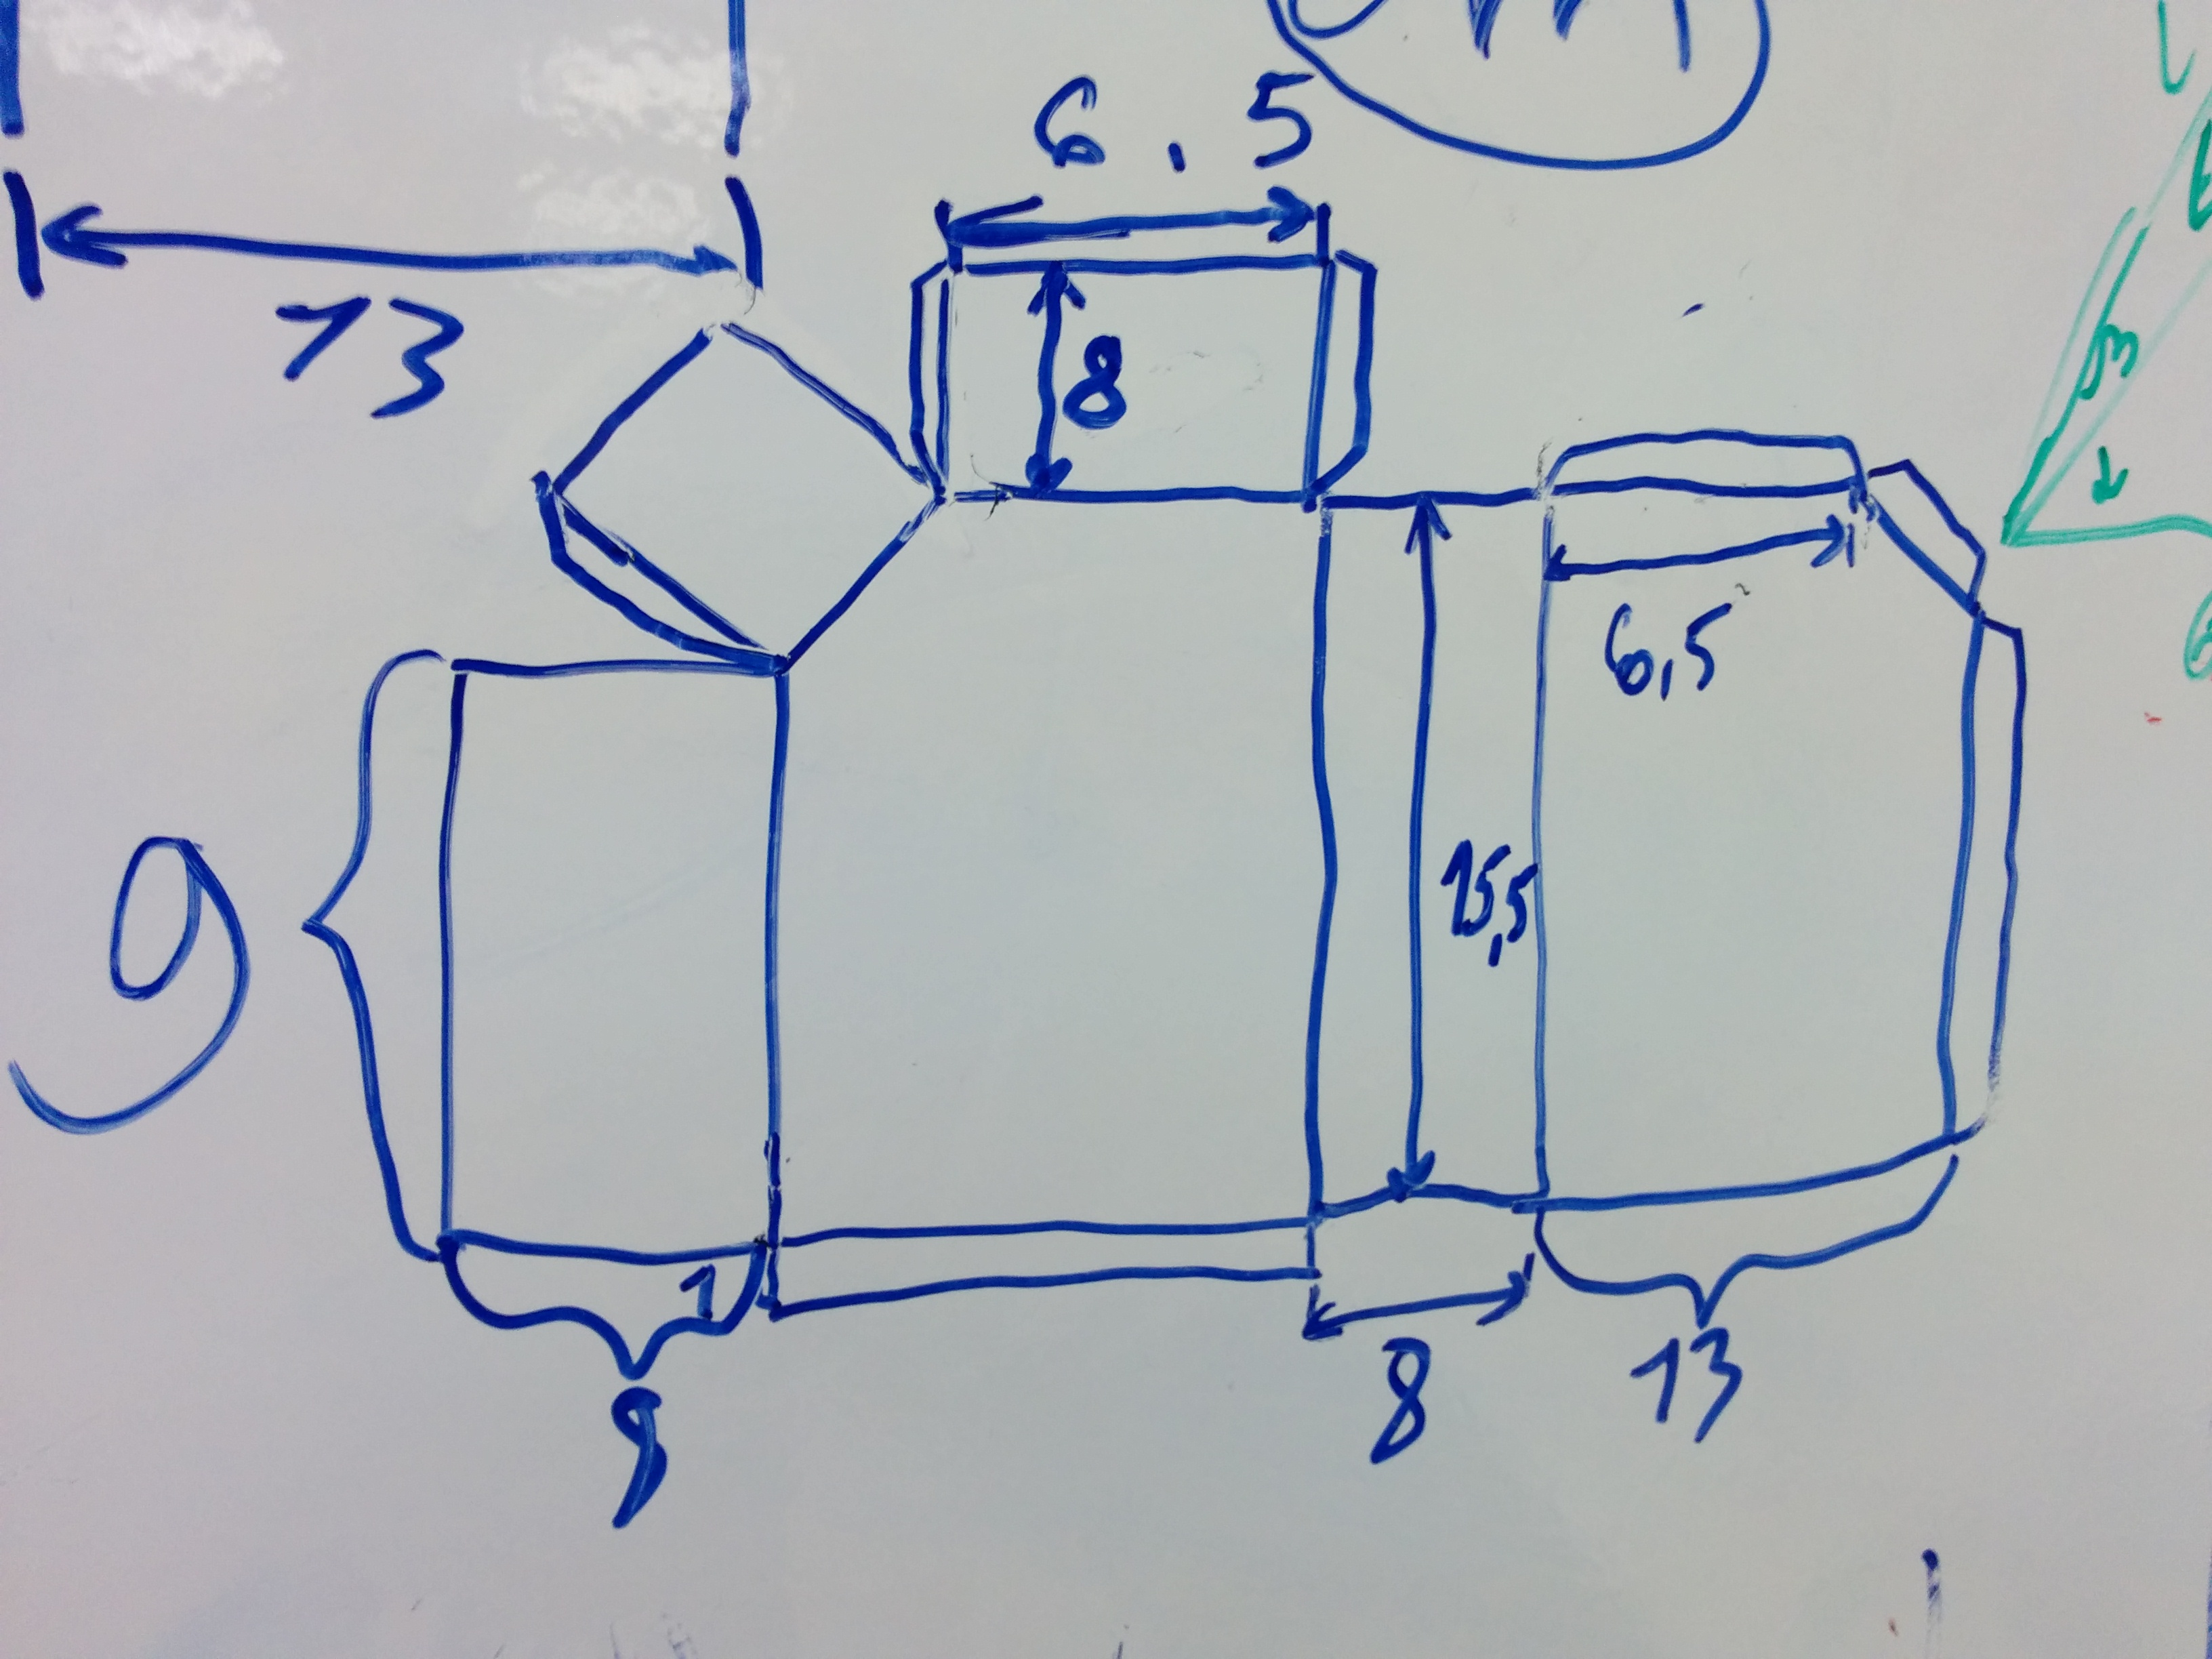
\includegraphics[scale = 0.05]{3Engineering/6Specifications_for_modules/bucket/images/12}}
  	\caption{Closer view of the scan}
  \end{minipage}
 \end{figure}
  
  This shape was chosen because: 
  \begin{itemize}
  	\item It was easier to fill by the gripper
  	\item It was big enough to hold 5 cubes
  	\item It was not enough spacious for 6 cubes
  	\item It has output hole with width of 2 cubes and that made cube falling vore direct and allows to score cubes.  
  \end{itemize}
  \item Then the new bucket was marked and cut from a sheet of plastic (the same was used for the first bucket). Next, bucket was assembled and tested (not on robot). Tests showed that bucket was able to hold 5 cubes and score them directly to the high scoring bucket. 
  
 \begin{figure}[H]
  \begin{minipage}[h]{0.49\linewidth}
  	\center{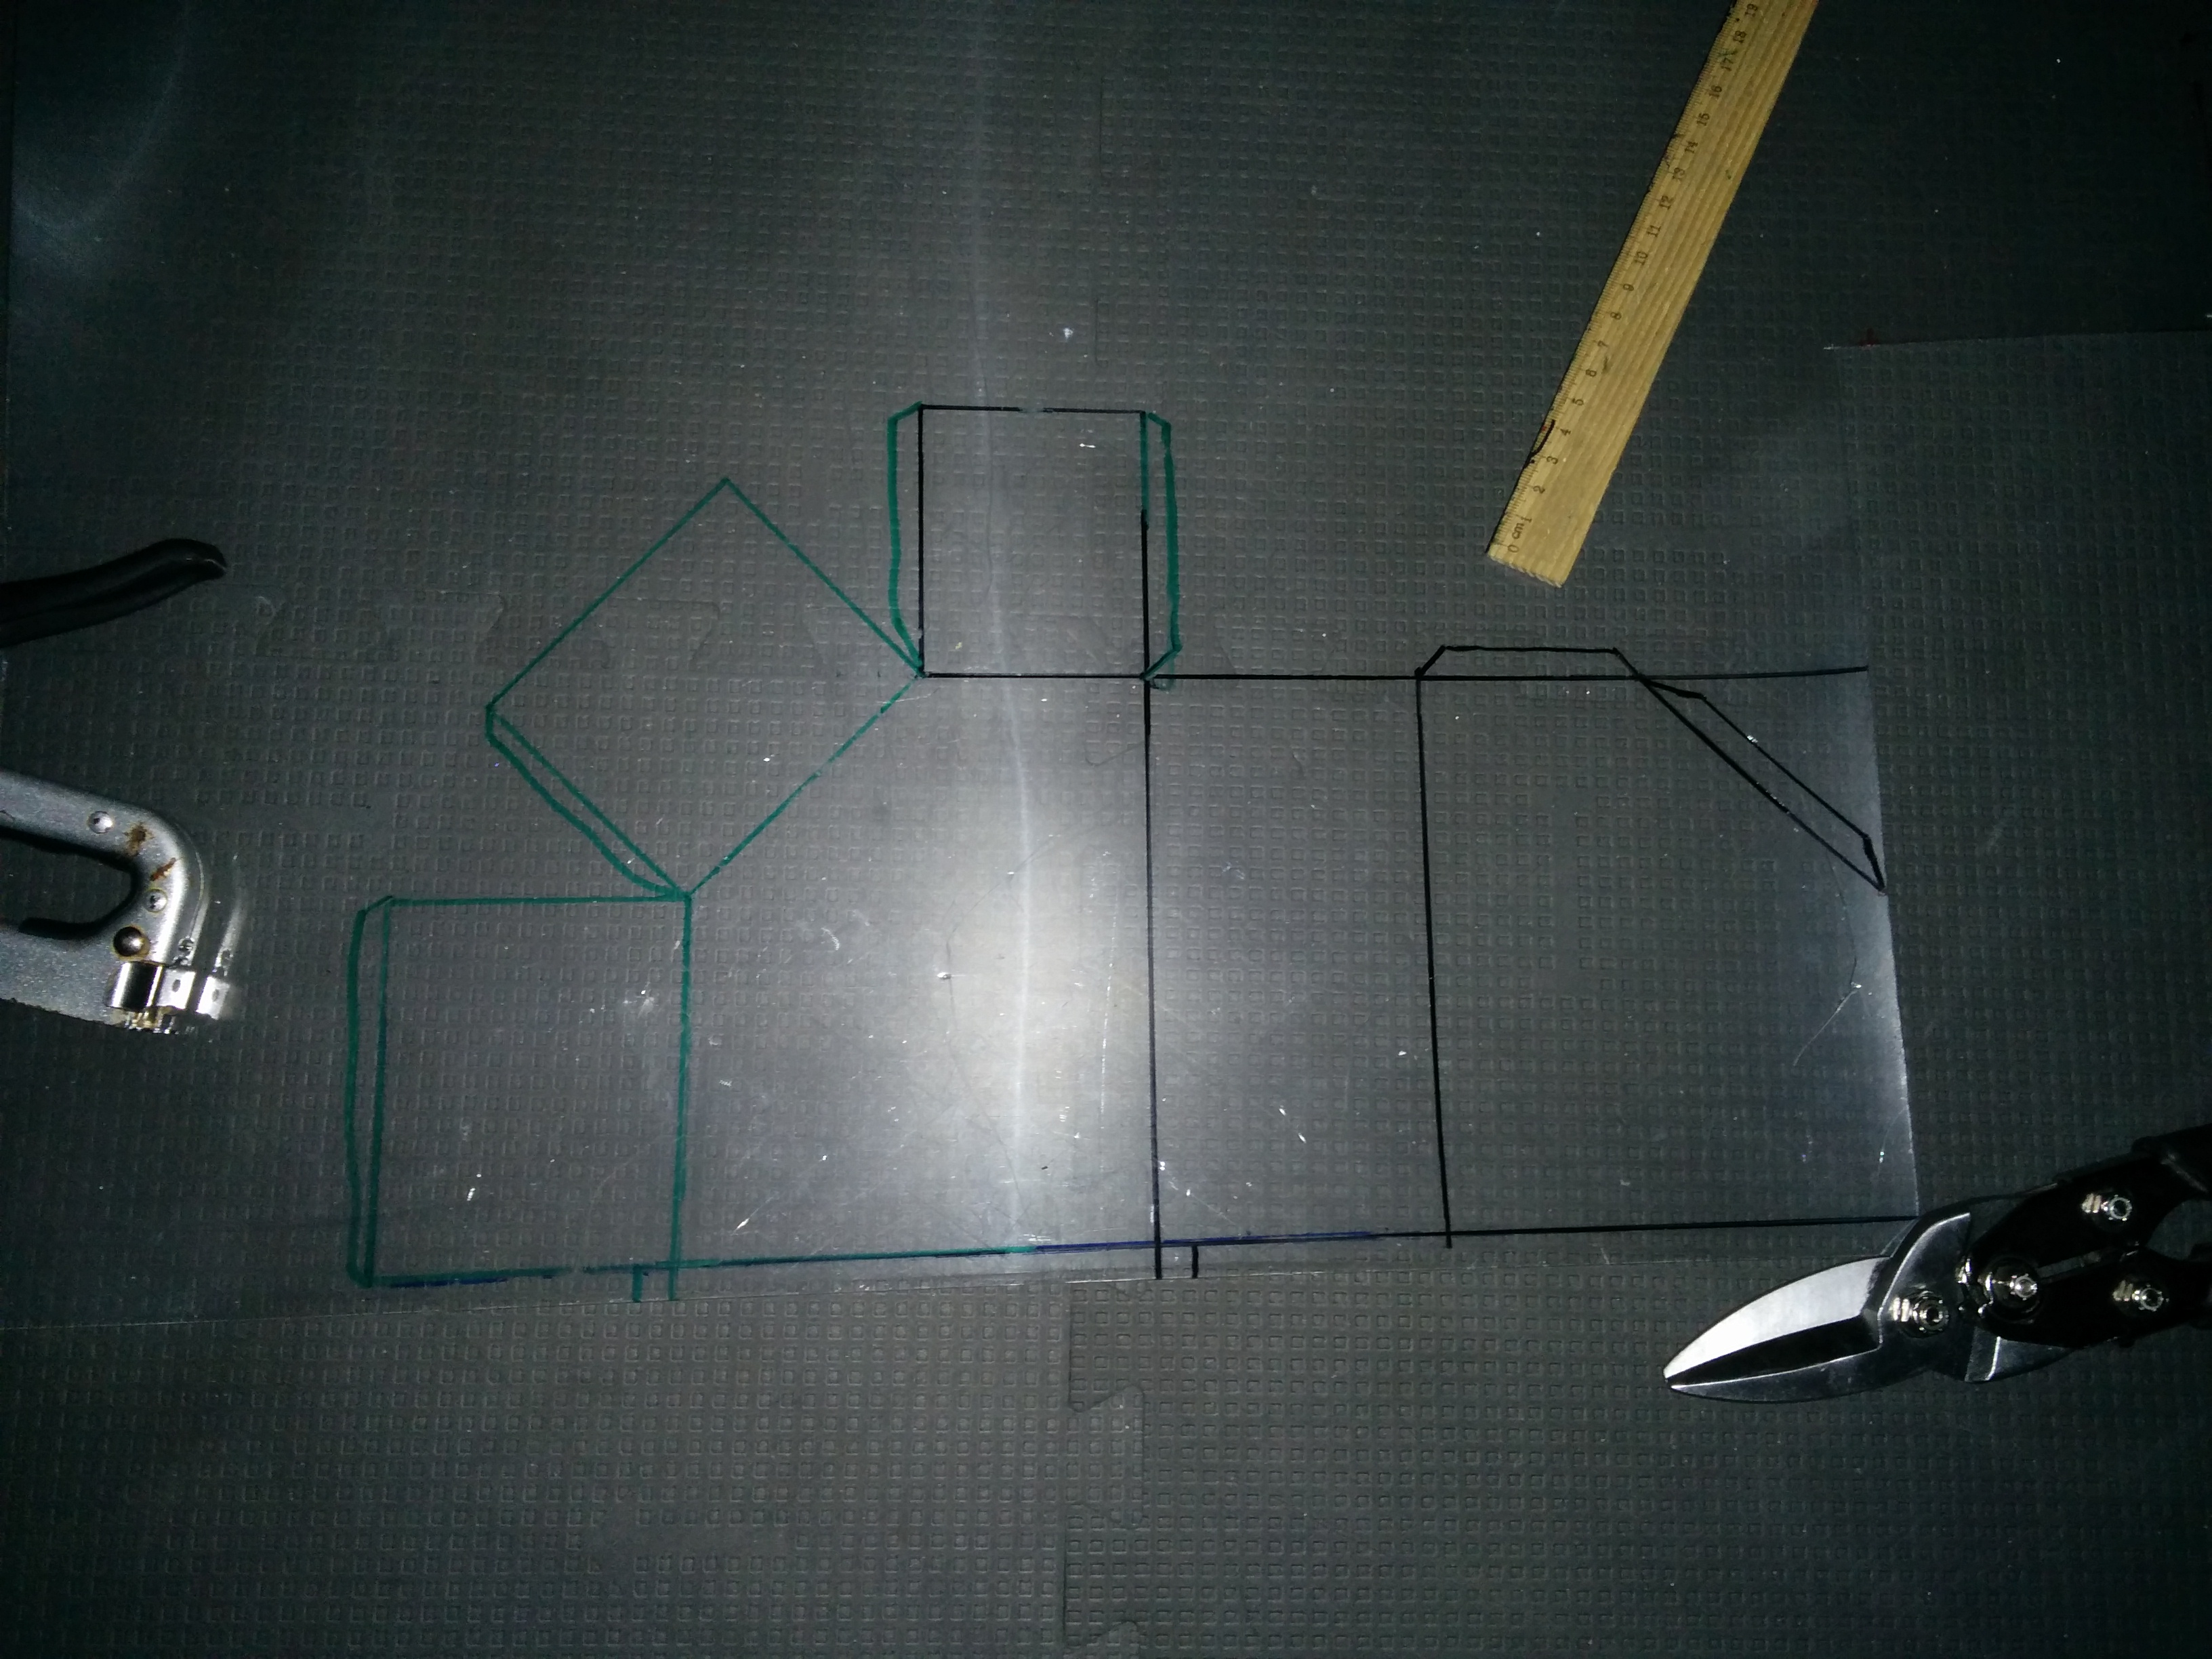
\includegraphics[scale = 0.05]{3Engineering/6Specifications_for_modules/bucket/images/13}}
  	\caption{Marking of bucket on the plastic sheet}
  \end{minipage} 
  \begin{minipage}[h]{0.49\linewidth}
  	\center{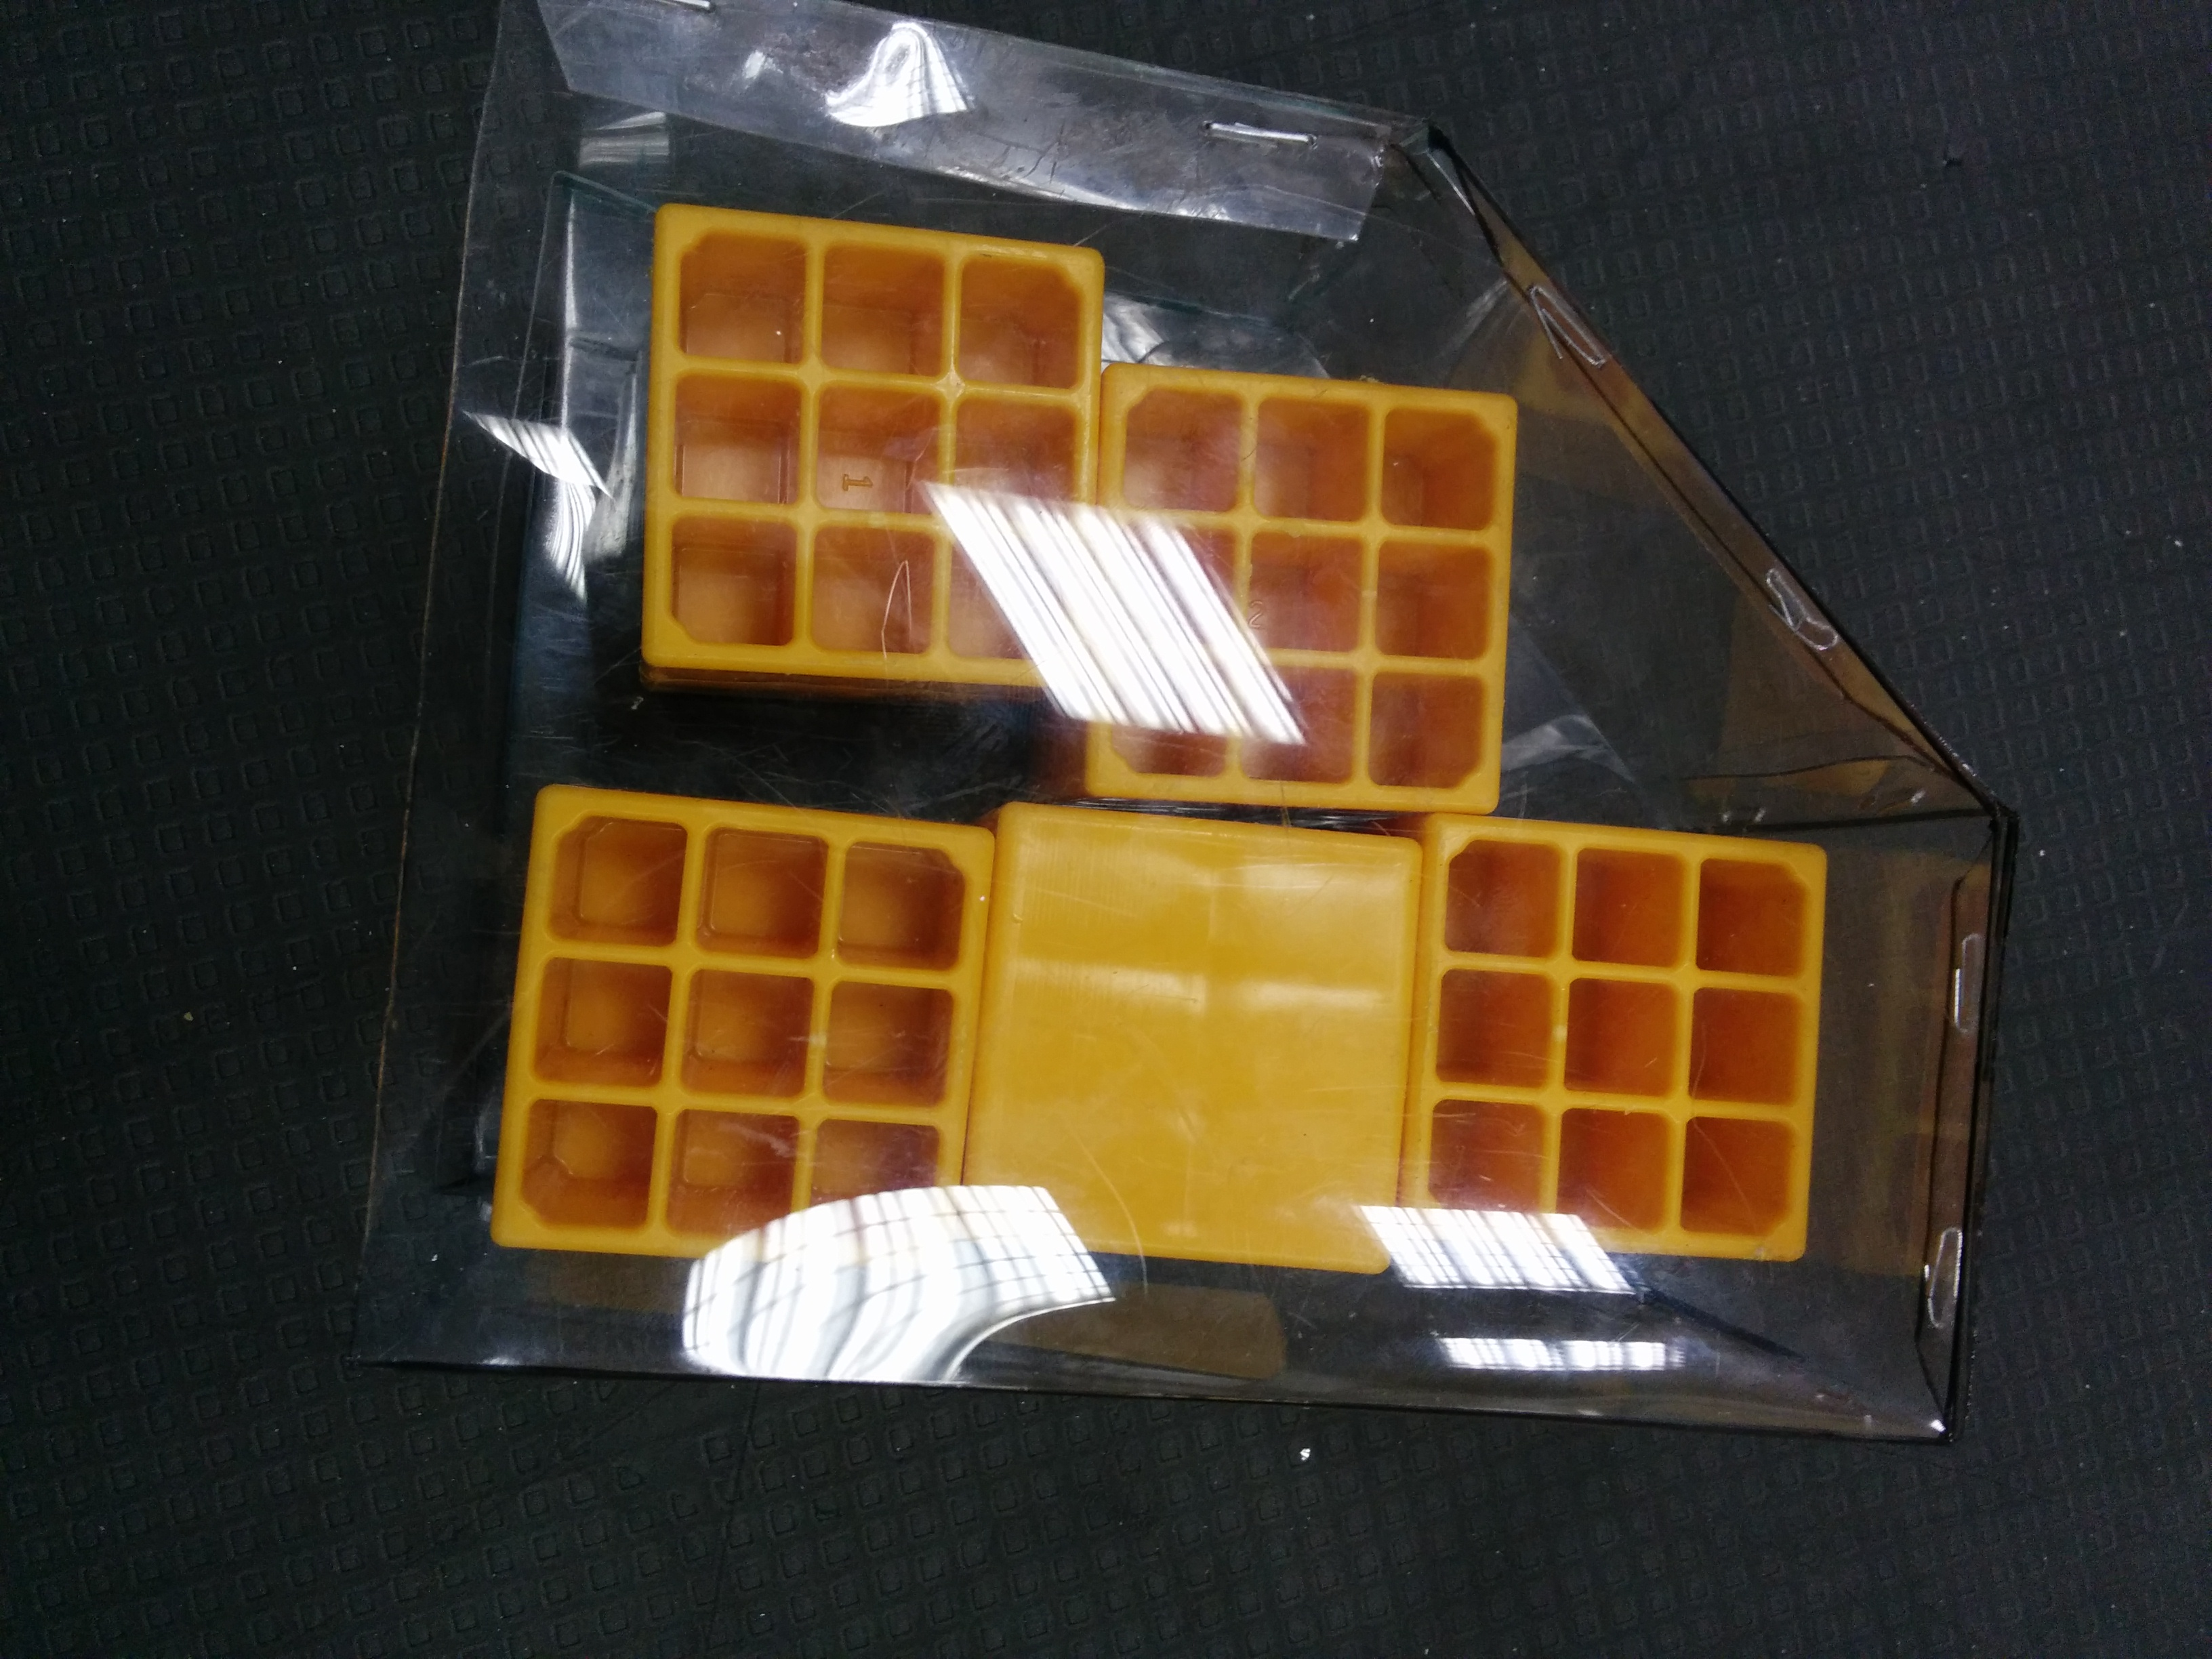
\includegraphics[scale = 0.05]{3Engineering/6Specifications_for_modules/bucket/images/14}}
  	\caption{Fully assembled bucket with cubes inside} 
  \end{minipage}
 \end{figure}
  
  \item After that was made protection for wires that could get into slats and break there. Also was made protection for rope of shifting mechanism that could catch on parts of robot because of which shifting stopped. Both protections are plastic strips.
  
 \begin{figure}[H]
  \begin{minipage}[h]{0.49\linewidth}
  	\center{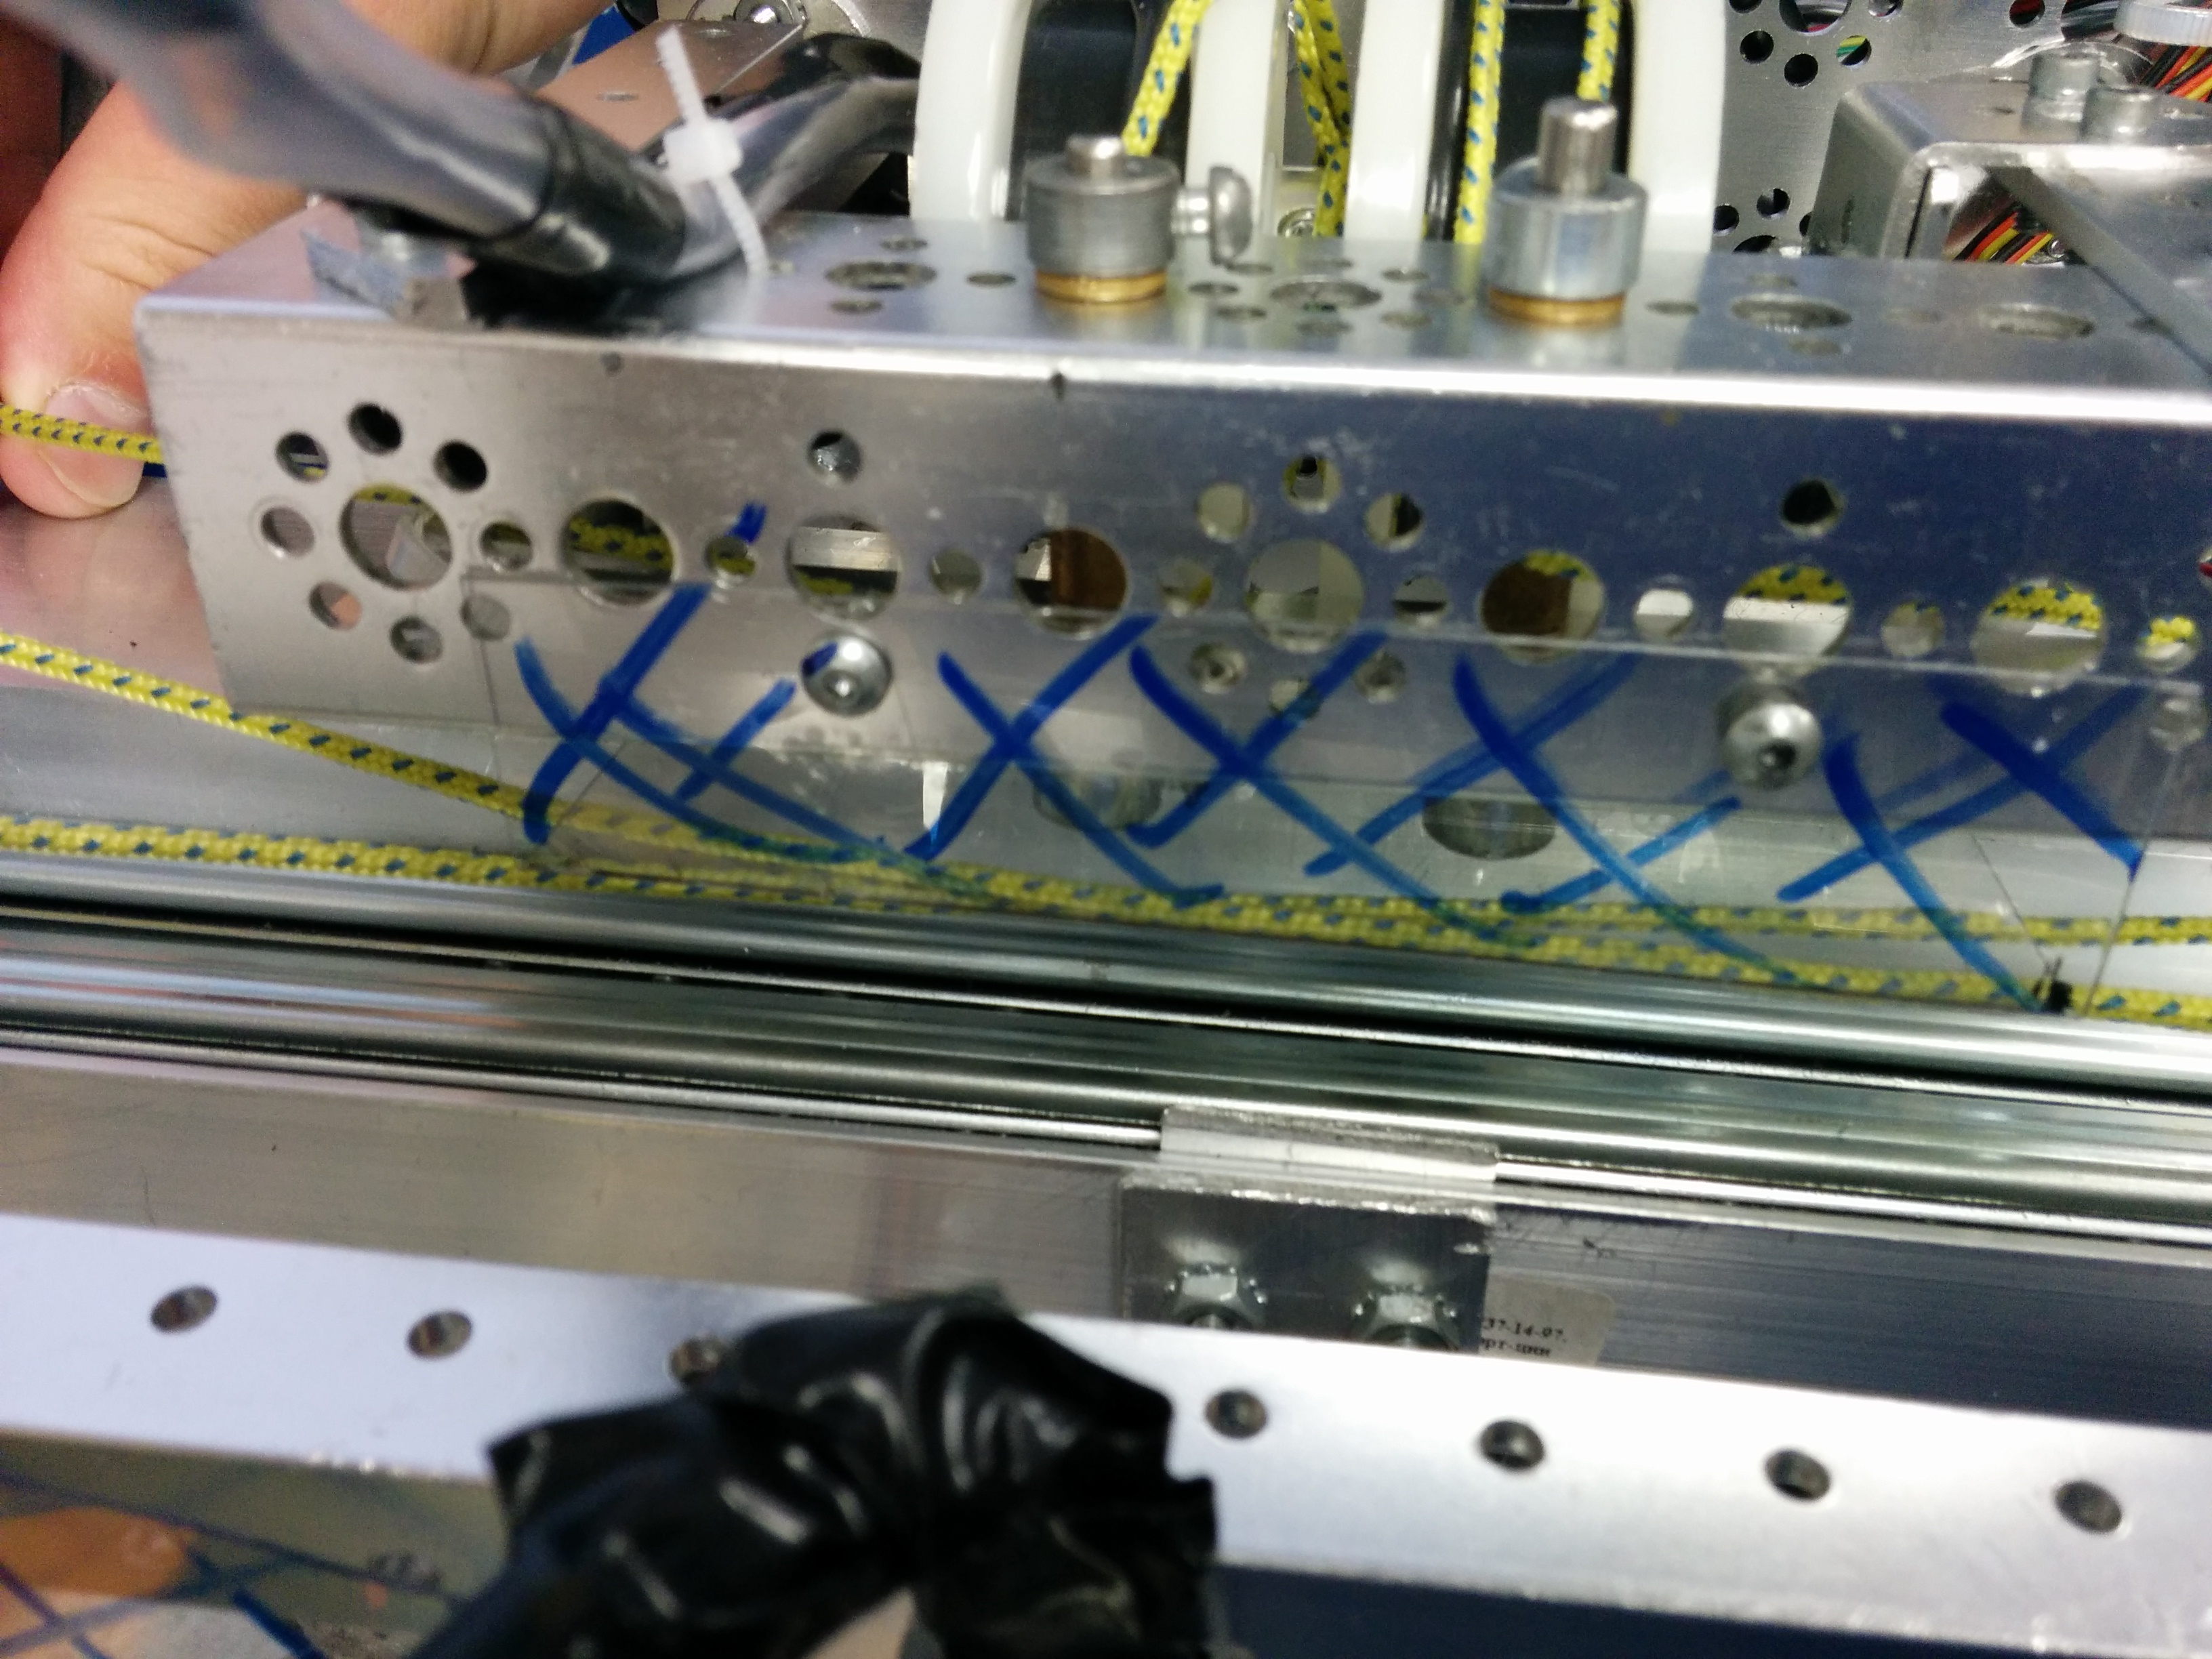
\includegraphics[scale = 0.05]{3Engineering/6Specifications_for_modules/bucket/images/15}}
  	\caption{Protection of rope}
  \end{minipage} 
  \begin{minipage}[h]{0.49\linewidth}
  	\center{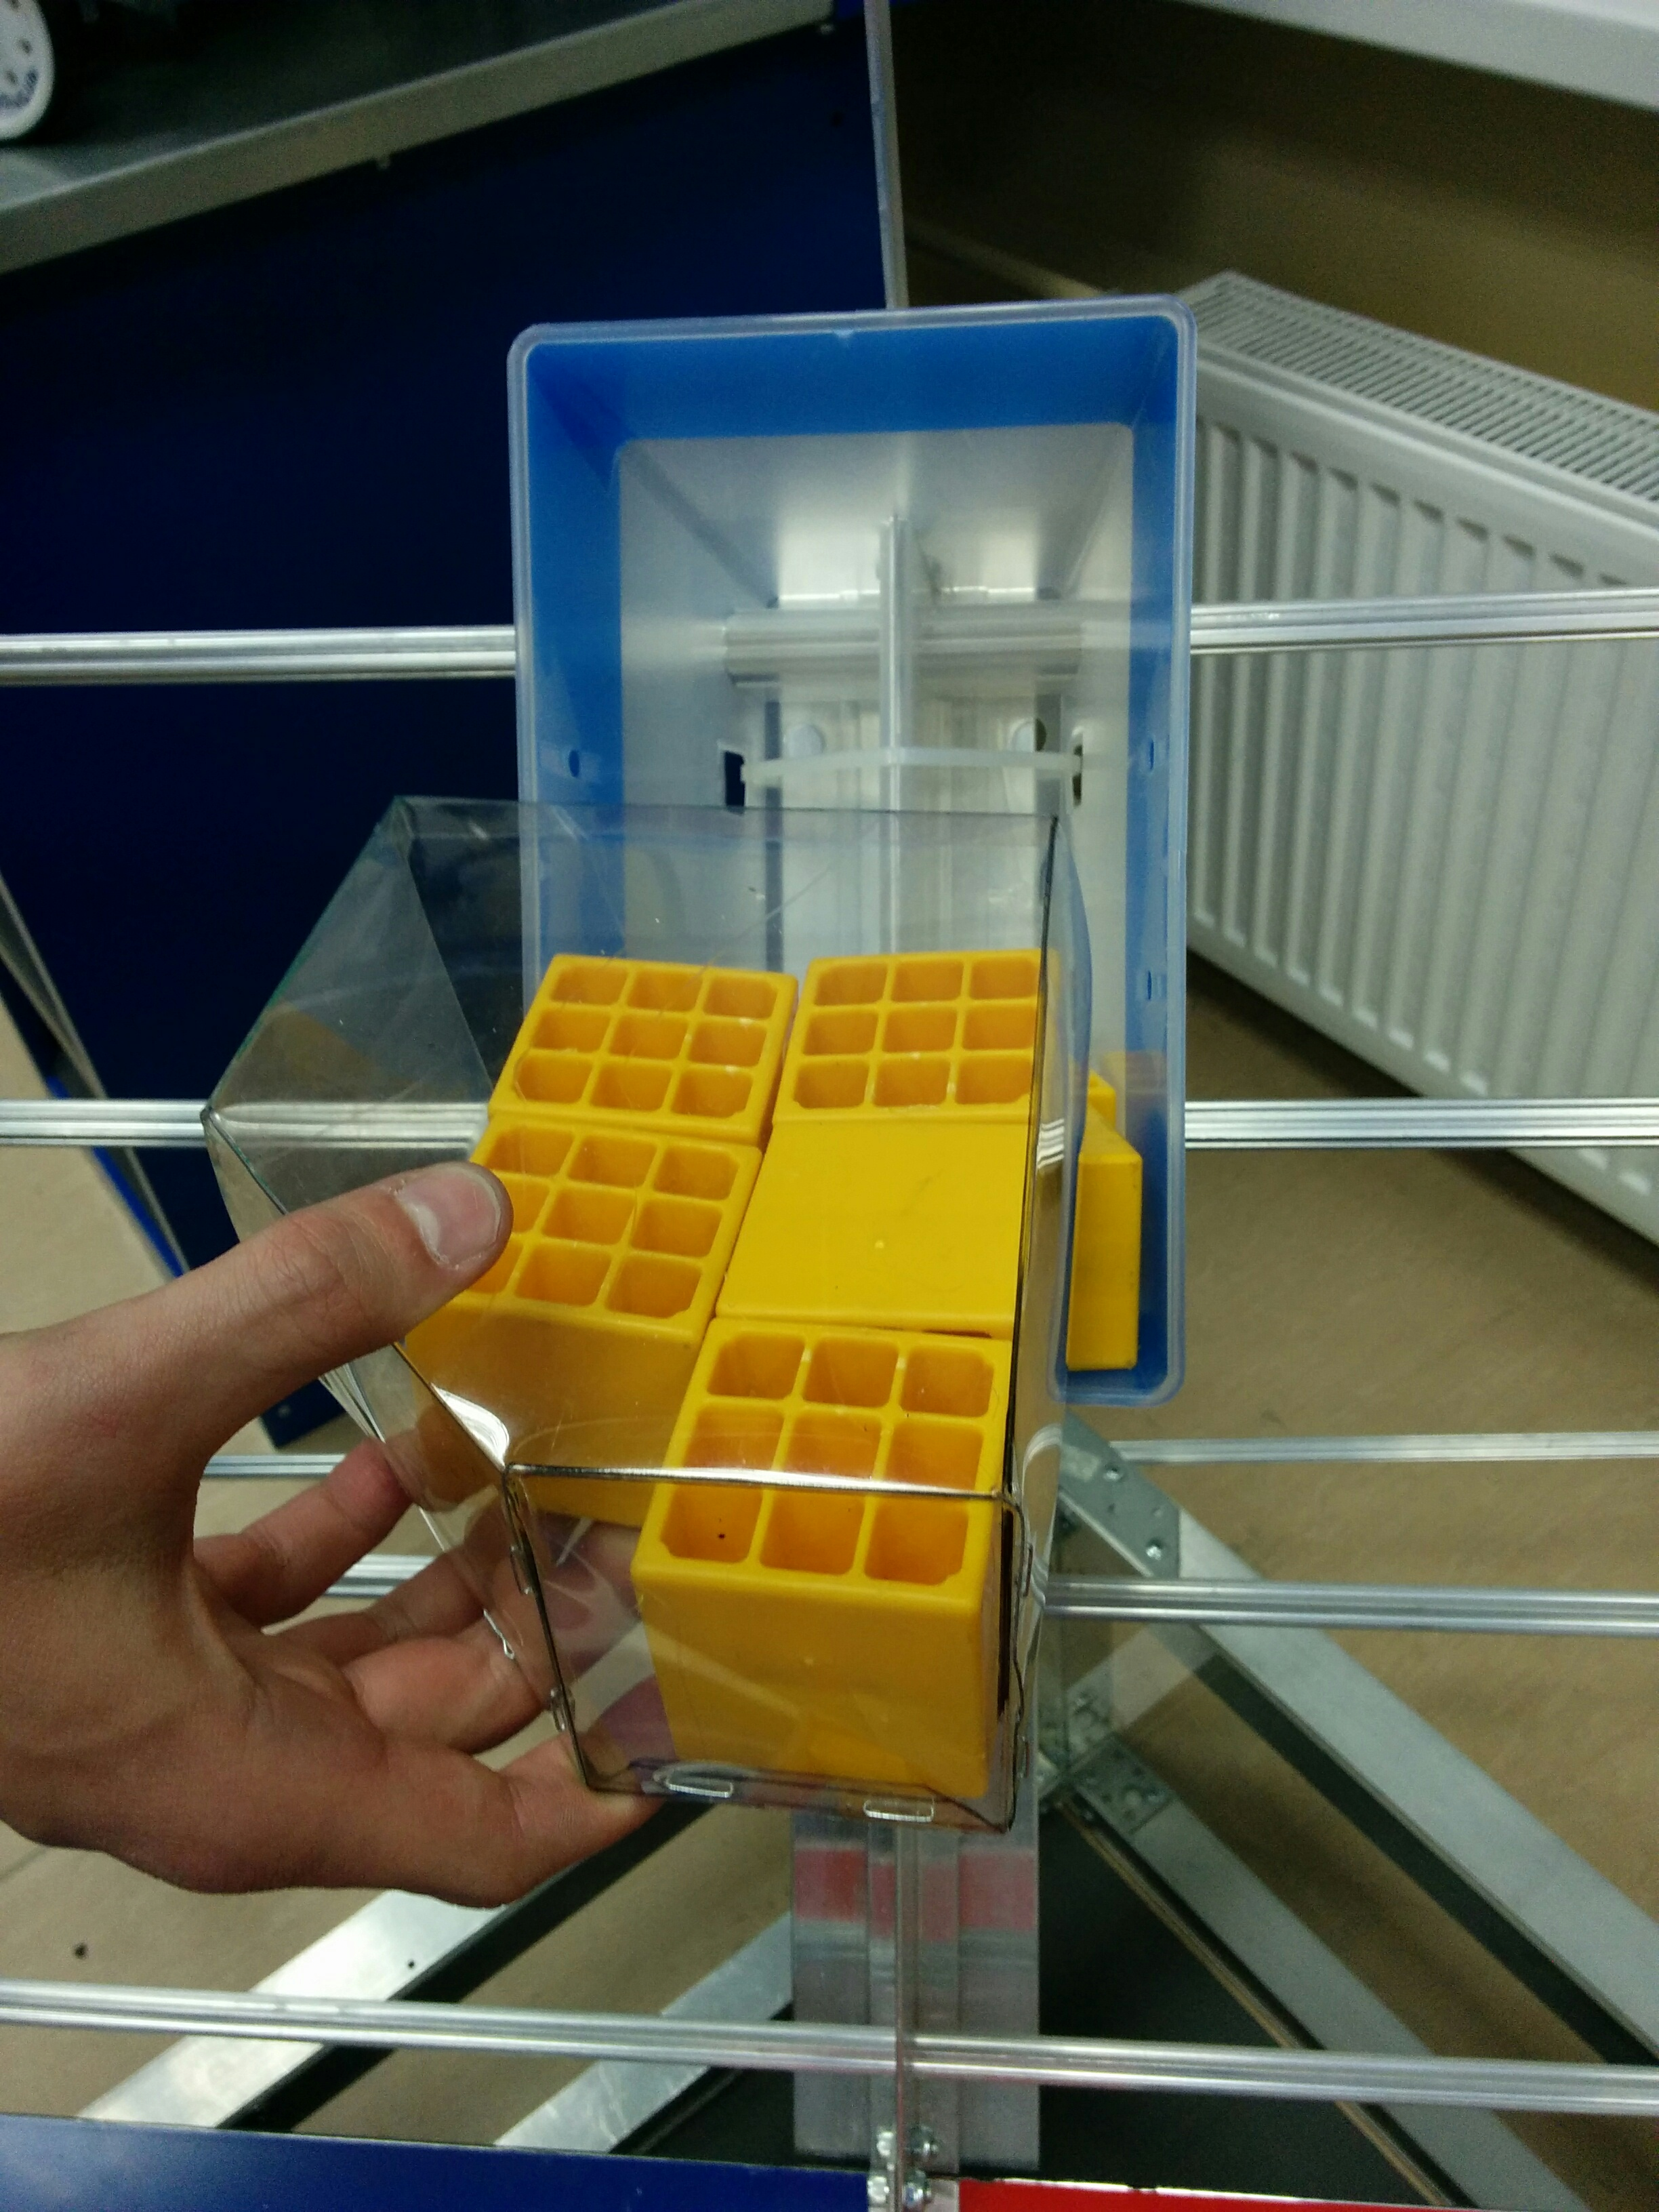
\includegraphics[scale = 0.05]{3Engineering/6Specifications_for_modules/bucket/images/16}}
  	\caption{Test of new bucket}
  \end{minipage}
 \end{figure}
  
 \item Then competitions FTC Russia Open in Sochi started and no more upgrades were done but the cutting off part of cover of the bucket. It was made in order to make cover not be inside the scoring goal while dropping debris into it. This made process of scoring much more fast, safety and easy for operators.
 
 \item After the competitions was made a decision on the creating new structure of robot and fully rebuilding it with making models of modules in CREO first. In new construction bucket wouldn't turn and had to have 2 holes: for debris entering on the top and for their falling on the bottom. It had to be spacious enough to let balls go throw it freely. New shifting mechanism had to be the same with some new features: two directions slat instead of two slats, lighter and easier mechanism of coiling the rope.
 
 \item In the process of designing new shifting mechanism was decided to use wheel and rope from jalousie. It makes all mechanism much smaller and lighter. Servo had to be the same but with the gear to make shifting faster. it was decided to use lego gears because of their small weight and easy mounting.   
  
   \item The model of shifting mechanism with 1 slat was made in CREO. 
   \begin{figure}[H]
     \begin{minipage}[h]{0.49\linewidth}
 		\center{\includegraphics[scale = 0.05]{3Engineering/6Specifications_for_modules/bucket/images/17}}
 		\caption{Shifting mechanism in CREO}
 	 \end{minipage} 
 	 \begin{minipage}[h]{0.49\linewidth}
 		\center{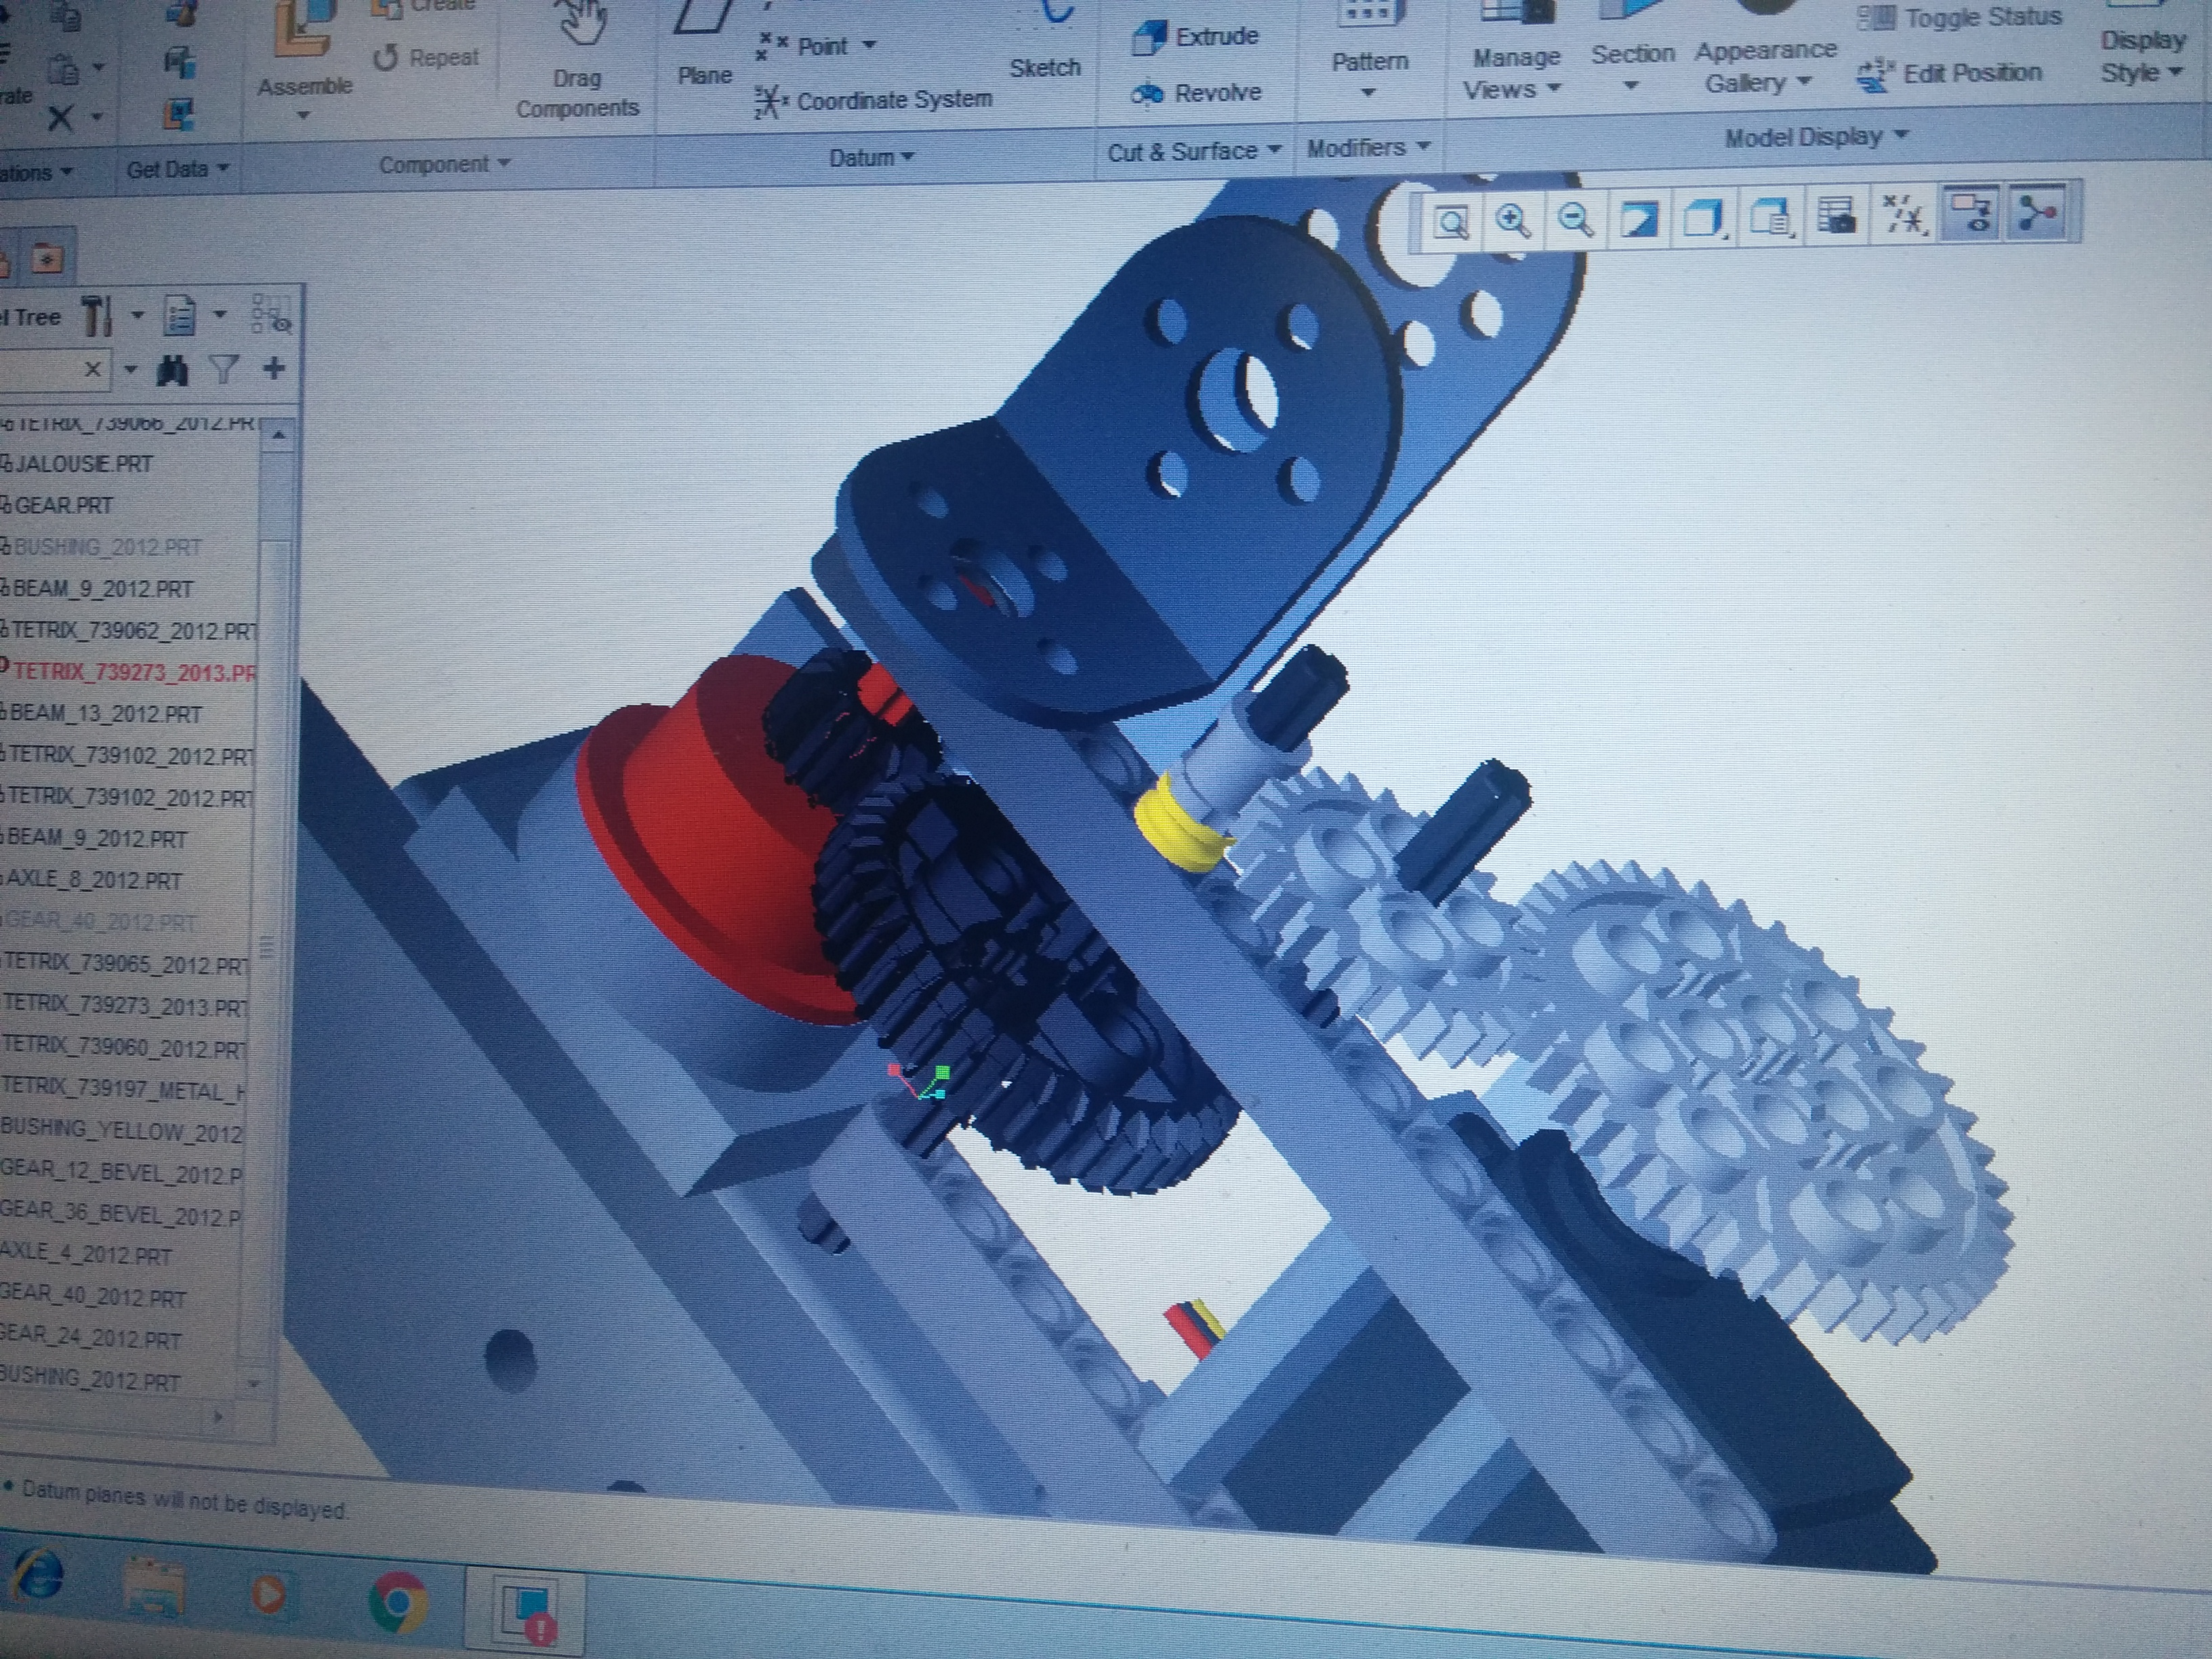
\includegraphics[scale = 0.05]{3Engineering/6Specifications_for_modules/bucket/images/18}}
 		\caption{Shifting mechanism in CREO}
 	 \end{minipage}
   \end{figure}
 
 \end{enumerate}	

\fillpage